%PoWeReD bY aKhIlEsH a. (Power Electronics 2015-17, M.A. College of Engineering, Kothamangalam)
\documentclass[12pt,a4paper]{report}
%thanks for using LATEX
%Please contact the department to report spelling mistakes or bugs
%Please do not make changes to the main template code without the consent of the HOD, Dept. of Computer Science \& Engineering
\date{}
\usepackage[hmargin={1.15in,1in},vmargin={1in,1.1in},]{geometry}
%\usepackage[hmargin={1.5in,1.25in},vmargin={1in,1in},]{geometry}
\usepackage{amsmath,graphicx,makeidx,listings,subfigure,float,setspace}
\usepackage{mathptmx}
\usepackage{fancyhdr}
\thispagestyle{empty}
\usepackage{sectsty}
\usepackage{lipsum}
\usepackage[toc,page]{appendix}

%\usepackage[center]{titlesec}
\usepackage[final]{pdfpages}
\usepackage{titlesec}
\renewcommand\contentsname{\Large \begin{center} {CONTENTS} \end{center}}
\renewcommand\listfigurename{\Large \begin{center} {LIST OF FIGURES} \end{center}}
\renewcommand\listtablename{\Large \begin{center}{LIST OF TABLES} \end{center}}

%\renewcommand\thebibliography{THEBIBLIOGRAPHY}
%---------------------------------FRONT PAGE--------------------------------------------------------------
\title{{\bf \Huge Digital Menu Cards for Restaurants and Ordering System
Using QR Code Scanning }\\    
\vspace{0.5cm}
{\normalsize {PROJECT REPORT}}\\
\vspace{0.15cm}
{\normalsize{ submitted by}}\\
\vspace{0.30 cm}
{\textbf{\large{ ARUN PRAKASH {\normalsize (Reg. No : PJR16CS015)}}}}\\
{\textbf{\large{ ATHIRA MANIYAN {\normalsize (Reg. No : PJR16CS017)}}}}\\
{\textbf{\large{ HASHIM M. {\normalsize (Reg. No : PJR16CS020)}}}}\\
% {\textbf{\large{ NAME4 {\normalsize (Reg. No : PJR15CSxxx)}}}}\\
%
\vspace{0.5cm}
\normalsize{to}\\ 
\vspace{0.2cm}
\normalsize {\bf APJ Abdul Kalam Technological University}\\
\vspace{0.2cm}
\normalsize {in partial fulfillment of the requirements for the award of the Degree}\\
\vspace{0.2cm}
\normalsize {of}\\
\vspace{0.2cm}  
\vspace{0.2cm}
{\normalsize {\textbf {\textit {Bachelor of Technology}} }\\ in \\ {\textbf {Computer Science and Engineering}}}\\
\begin{figure}[H]
\centering

\includegraphics[scale=0.05]{emblem}
\end{figure}
{\large \textbf {Department of Computer Science and Engineering}}\\
\vspace{0.2cm}
{\large \textbf {College of Engineering Poonjar}}\\
\vspace{0.2cm}
\normalsize {Poonjar Thekkekkara P O, Kerala, India 686582}\\
\vspace{0.35cm}
\author \large {MAY 2020}}
%----------------------------------TABLE OF CONTENTS DEPTH-----------------------------------------------
%\setcounter{tocdepth}{1}
\renewcommand{\bibname}{\Large REFERENCES}
%-------declaration-----------------------------------------
\begin{document}
\maketitle
\vspace*{1.3in}
\begin{center}
\large \textbf{DECLARATION}
\end{center}
\thispagestyle{empty}
\onehalfspacing
\par I undersigned hereby declare that the project report ``\textbf{Digital Menu Cards for Restaurants and Ordering System
Using QR Code Scanning}", submitted for partial fulfillment of the requirements for the award of degree of Bachelor of Technology of the APJ Abdul Kalam Technological University, Kerala is a bonafide work done by me under supervision of \textbf{Mrs. Saira Shamsudeen}, Assistant Professor, Dept. of  Computer Science \& Engineering, College of Engineering Poonjar. This submission represents my ideas in my own words and where ideas or words of others have been included, I have adequately and accurately cited and referenced the original sources. I also declare that I have adhered to ethics of academic honesty and integrity and have not misrepresented or fabricated any data or idea or fact or source in my submission. I understand that any violation of the above will be a cause for disciplinary action by the institute and/or the University and can also evoke penal action from the sources which have thus not been properly cited or from whom proper permission has not been obtained. This report has not been previously formed the basis for the award of any degree, diploma or similar title of any other University.
\vspace {0.25 in}
\begin{flushleft}
Poonjar \\ 
6/05/2020  \hfill{{\textbf{Arun Prakash}}} \\
\hfill{{\textbf{Athira Maniyan}}} \\
\hfill{{\textbf{Hashim M.}}}
\end{flushleft}
%-----------------------------------CERTIFICATE-----------------------------------------------------------
%Dont Break Your Name Over Two Lines
%\begin{document}
\newpage
%\begin{doublespace}
\begin{center}
{\large \bf{DEPARTMENT OF COMPUTER SCIENCE AND ENGINEERING}}\\
\vspace{0.35cm}
{\large \bf{COLLEGE OF ENGINEERING POONJAR}}\\
\vspace{0.35cm}
\end{center}
%\end{doublespace}
\begin{center}
\thispagestyle{empty}

\includegraphics[scale=0.05]{emblem}\\[7pt]
\large{\bf{CERTIFICATE}}
\end{center}
\vspace{0.50cm}
\onehalfspacing 
This is to certify that the report entitled {\large{ \textbf{Digital Menu Cards for Restaurants and Ordering System
Using QR Code Scanning}}} submitted by \textbf{Ms. Athira Maniyan (PJR16CS017)} to the APJ Abdul Kalam Technological University in partial fulfillment of the requirements for the award of the Degree of Bachelor of Technology in Computer Science and Engineering is a bonafide record of the project work carried out by him under our guidance and supervision. This report in any form has not been submitted to any other University or Institute for any purpose.
\vspace{1in}
\begin{flushleft}
\textbf{Saira Shamsudeen} \hfill \textbf{Mr. Rajesh K R}\\ 
\textbf{Project Guide}  \hfill{\textbf{Head of Department}}\\
\textbf{Asst. Prof. of Computer Science} \hfill{\textbf{Computer Science}}\\
\textbf{College of Engineering Poonjar}\hfill{\textbf{College of Engineering Poonjar}}
\end{flushleft}

\tableofcontents


  %--------------------------------------ACKNOWLEDGMENT------------------------------------------------
\newpage
\pagenumbering{roman}
\setcounter{page}{1}
\addcontentsline{toc}{chapter}{\MakeUppercase{ACKNOWLEDGMENT}}
\begin{verbatim}
\end{verbatim}
\begin{center}
\textbf {\large ACKNOWLEDGEMENT}
\end{center}
\vspace{0.4125in}
\par
It is a great pleasure to acknowledge all those who have assisted and supported me for successfully completing my project.
\\
\par 
First of all, I thank God Almighty for his blessings as it is only through his grace that I was able to complete my project successfully.
\\
\par 
I take this opportunity to extend my sincere thanks to my project guide \textbf{Mrs. Saira Shamsudeen}, Assistant Professor, Dept. of  Computer Science, College of Engineering Poonjar for her constant support and immense contribution for the success of my project.
\\
\par
I also extend my sincere thanks to all other members of the Department of  Computer Science \& Engineering for sharing their valuable comments  during the preparation of the project.
\\
\par
I am also grateful to \textbf{Prof. Rajesh K. R.}, Project Coordinator and Head of Computer Science \&  Engineering Department, for the valuable guidance as well as timely advice which helped me a lot during the preparation of the project.
\\
\par
I am deeply indebted to \textbf{Dr. E S Jayachandran}, Principal, College of Engineering Poonjar for his encouragement and support.
\\
\par
 I whole - heartedly thank all my classmates, for their valuable suggestions and for the spirit of healthy competition that existed between us.
%-----------------------------------------ABSTRACT--------------------------------------------------------
\newpage
\addcontentsline{toc}{chapter}{\MakeUppercase{Abstract}}
\begin{verbatim}
\end{verbatim}
\begin{center}
{\bf \Large {ABSTRACT}}
\end{center}
\vspace{30pt}
\begin{doublespace}
\par
An entirely new concept in the food industry is being introduced through this project. Our project "\textbf{Digital Menu Cards for Restaurants and Ordering System
Using QR Code Scanning}" is an entirely new system to handle the ordering systems inside an hotel or restaurants. This project offers an efficient ordering system for the hotels and restaurants. Our Online Restaurants Menu Card System helps you to Streamline your
operations to meet customer’s expectations.
A flexible restaurant manage system which helps you to be more systematic and
quick in your services to customers.
Its fast and time management system for customers and as well as the hotel management.
\\
\\
\par
The entier project is develpoed using Django and deployed in heroku. The storage space required while deploying the project is acquired using Amazon Web services. Some features of the project has been developed using java. The QR Code and Add-Ons are the applications of java. The proposed system has following modules incroporated in it. They are User Module, Food Item Management Module, Category Module, Confirm Order Module, Payment Module, Comment Module and Rating Module
\end{doublespace}

%%-----------------------------TABLE OF CONTENTS-----------------------------------------------------------
%\newpage
%{
%%\includepdf[pages={1}]{contents}
%}
%%\listoftables
%\addtocontents{lot}{ \hspace{0.4cm} No. \hspace{1in} Title \hfill{Page No.}\par}
%%\listoffigures
%\addtocontents{lof}{ \hspace{0.4cm} No. \hspace{1in} Title \hfill{Page No.}\par}
\newpage
\addcontentsline{toc}{chapter}{LIST OF TABLES}
\listoftables
\newpage
\addcontentsline{toc}{chapter}{LIST OF FIGURES}
\listoffigures
%----------------------HEADER AND  FOOTER-----------------------------------------------------------------
\newpage
\pagenumbering{arabic}
\setcounter{page}{1}
\pagestyle{fancy}
\lhead{\emph{Digital Menu Cards for Restaurants and Ordering System
Using QR Code Scanning  }}
\chead{}
\rhead{}
\lfoot{\emph{Dept. of Computer Science \& Engineering, CE Poonjar}}
\cfoot{}
\rfoot{\thepage}
\renewcommand{\headrulewidth}{1pt}
\renewcommand{\footrulewidth}{1pt}
\renewcommand{\chaptername}{ \Large{CHAPTER}}
%\renewcommand{\cftchapfont}{16pt}
\chapterfont{\centering}
\renewcommand\bibname{REFERENCES}
%------------INTRODUCTION---------------------------------------------------------------------------------

\chapter{INTRODUCTION}
\hspace{0.25cm}
\par
 With increasing population, there has been a drastic
increase in their demands and everyone is running out of
time. The fact of significance is that no one wants to waste
their time in long queue to get their task done . Usually one
has to wait for a very long time to get their job done may be
because of multiple load on the system receiving and
processing the task or due to first-come first-serve approach
which hinders those who have higher priority task to be
done first but late to put request for execution. This
problem is faced by a lot of organizations that still have the
primitive processing system and also at a lot of places that
are still dependent on manual work for processing requests.
\\
\\
\par
There has not been much of advanced concept introduced in a
lot of sectors that have a really good chance to bloom if
they have the help of advanced technologies to attract more
people and attention and hence a lot more profits. Since
technology is always advancing, we can deploy it in real
time applications to maximize the performance of the
service systems and make it optimal.
\\
\\
\par
The connectivity between the systems have not seen
much advancement either when implemented in real world,
the information transfers have always been happening in
the old fashioned manner involving a lot of congestion and
attenuation. There are chances that the request may enter in
a deadlock situation if there is a collision of request
initiating from the two or more consumers, and hence
failing the system's throughput. The different sites that
have installed a good communication system are facing the
problem of network congestion, involving a lot of requests
at the same time and no proper algorithm to regulate the
requests and hence the quality of service deteriorates
eventually causing packet loss, request delay and also
blocking of new connections 
\\
\\
\par
There are some places where manual system is still
considered a good option over automated systems for better
interaction with the user and proper understanding of the
situation, but the time factor is often ignored in such cases.
There are areas that require immediate transfer of
information and hence manual system is not a good choice.
Also these areas are reluctant to adopt the new system due
to high cost of the existing systems and hence they haven't
implemented much advancement in their existing systems.
On one side where manual systems are slow and there
always is a scope for human errors, there lies automated
systems on the other side that are fast, more informative for
the users and also keeps record of all the processes and
hence there is a very less scope for errors.
\\
\\
\par
This Digital Menu Card System has been developed to override the problems prevailing in the manual orderin systems. This software eliminates and reduces the hardship faced in the exi manual systems.Moreover this is developed particularly for smooth and efficient functioning of the administration. 
\\
\\ 
\par
This application possibly reduces the error of serving wrong orders to the customers. No formal knowlegde is required to use this software. It is a user-friendly. The main objective of this application is an efficient management of deatils of Food item, cart, category, order, customer. It manages all the informations securely. the project is totaly built on administrator's end and thus only administrator is gauranted access.
% \\
% \\
% For this problem to be solved , there is need for proper and effective metering systems. If such metering systems are installed, there is also need for constant monitoring of the meter to know when the consumer has tampered with it or when the consumer has bypassed it. This will require the staff of the distribution companies to constantly visit the premises of the consumer for both meter reading and tamper activity inspection; this is a lot of work for the staff and not feasible. 
%  \\
%  \\
%  So an attempt is made to prevent electricity theft by making a meter to be tamper proof.The primary objective of this study is to develop an  Electricity Theft Detection Prevention using GSM concept.
%  \\
%  \\    
%  If electricity theft is curbed, there will be an improvement in the power sector. There will be reduction in electricity tariff and the electricity companies (distribution, transmission and generation) will make enough profit and begin to plan for expansion of their businesses. For example, if the Generation companies expand their businesses, it means that more power will be generated and supplied to the Transmission Company. At the end of the day, there will be an increase in the amount of power available for the consumers to use.Traditional meter reading by human operator is inefficient to meet the future residential development needs.Collection of meter readings becomes more problematic and costly when readings have to be collected from vast, and often scattered rural areas.Meter readers are reluctant to make the effort to travel to such areas and will often submit inaccurate estimations of energy consumed.So there is increased demand for automatic billing system .So in addition to electric theft detection prevention we develops a energy billing system using GSM concept.
%  \\
%  \\ 
 %---------
%chapter1-------------------------------------------------------------------------------
\chapter{LITERATURE SURVEY}
\section{Online Food Ordering System - International Journal of Recent Technology and Engineering, Trupthi B, Rakshitha Raj R, J B Akshaya, Srilaxmi C P }
\hspace{0.25cm}
\par
An Online Food Ordering System is proposed
here which simplifies the food ordering process. The proposed
system shows an user interface and update the menu with all
available options so that it eases the customer work. Customer
can choose more than one item to make an order and can view
order details before logging off. The order confirmation is sent to
the customer. The order is placed in the queue and updated in the
database and returned in real time. This system assists the staff to
go through the orders in real time and process it efficiently with
minimal errors.
\section{Network Architecture for an Automated Service
System}
\hspace{0.25cm}
\par
Present Service Systems are very primitive and
time consuming where the customer has to first stand in the
long queue to place their order and then have to wait to
receive the order with uncertainty of amount of time to be
spent on processing their order/task. This paper proposes an
autonnted system that will enable customers to place the
orders at public service systems in a timesaving manner; the
custolller just needs to take the end handheld device which
can be any tablet or phone and order either online from home,
etc. making use of the central repository or using the local
server present in the premises. This will enable direct
processing of the task and the payment can be done in an easy
manner through the same end device.
The system will have one main server connecting all the peers
assuming more than one branch of the central system and also
the local server to provide services to the user sitting in the
System The customer will now get the status of the task done
as in how much is it processed and how much more time will it
take, a digital menu to select the options and also option to
pay from his card directly, hence saving a lot of time at every
point.
\section{A Study on E-Commerce Applying in Taiwan’s Restaurant Franchise}
\hspace{0.25cm}
\par
When Taiwan’s traditional food industry facing the
economic recession in 2008, except strengthen the
constitution of themselves, they also promote the
market scope to chain to develop franchise system
aggressively. In order to promote the competition of
enterprise and reduce management cost, this study that
the writer counseling ȸ LUNGHSIENCHU ȹ will
show the proven process of e-commerce, it becomes e-
commerce little by little including retail store
management, purchasing operation, service process,
customer relationship management and promote
management efficiency effectively. Then, they can
enlarge franchise chain, food chain e-commerce and
become operation model that can’t be held back.
\section{Research on E-commerce Mode of Food Enterprises}
\hspace{0.25cm}
\par
Food enterprises integrate supply chain management and e-commerce, in order to form complete e-supply chain. It is a better mode of promoting food businesses to develop rapidly. Food enterprises are rather unfamiliar with use of e-commerce for food enterprises, starting with the analysis of four stages of developinf e-commerce. With the analysis of advantages and deficiences of food enterprises developing e-commerce , the article discusses the objective requirementof food enterprises and proposes the counter measures based on the prsent situation of the food insudtry.  


% \\
% \\
% An IoT based embedded system that checks electricity theft and enables the remote control of appliance was presented in [8]. In this system, reference energy consumption is set and once the energy consumption rises above the threshold, the system considers the activity as electricity theft [8]. 
% \\
% \\
% In [9] G. L. Prashanthi, K. V. Prasad had proposed with GSM modules helps company to monitor the amount of usage by this specified costumer and generate bill periodically and send it to costumer via SMS, thus saving lot of labor work, time and cost of reading .The proposed found to be little bit complex as far as distribution network is concerned, but it’s an automated system of theft detection. It saves time as well as help to maximize profit margin for utility company working in electrical distribution network. 
% \\
% \\
% In paper[10] S.Anusha, M.Madhavi,R.Hemalatha had done the project model to reduces the manual manipulation work and theft. Use of GSM in our system provides a numerous advantages of wireless network system. The government saves money by the control of theft in energy meter and also more beneficial for customer side and the government side. The metering IC ensures the accurate and reliable measurement of power consumed. Cost wise low when compared to other energy meter without automatic meter reading and theft control.
% \\
% \\
%  In paper[11] Kalaivani. R, Gowthami. M, Savitha.S, Mohanvel.S had done the system, in which service provider can collect the bill any time with a single message. The data collection and manipulation task becomes fast and easier. Any modification can be made to the code in less time. Changes in rate or unit calculation can be done very effectively. The project model reduces the manual manipulation work and theft. Use of GSM in our system provide the numerous advantages of wireless network systems. The metering IC ensure the accurate and reliable measurement of power consumed. Hence we are trying to manipulate cost wise low when compared to other energy meter without automatic meter reading and theft control. 
% \\
% \\ 
%---------
%chapter2-------------------------------------------------------------------------------
\chapter{SYSTEM DESIGN}
\section{DISADVANTAGES OF THE EXISTING SYSTEM}
\begin{itemize}
	\item Time consuming process.
	\item Need of paper for printing menu cards.
	\item Need of more number of man power.
	\item More amount of manual work to be accomplished.
	\item Chances of serving wrong dishes to cutsomers.
	\item Lacks customer satisfaction.
	\item Daily Updates is not possible through printed menu cards.
\end{itemize}
\section{PROPOSED SYSTEM}
\hspace{0.25cm}
\par
The proposed system is an Digital Menu Card for ordering by scanning the QR Code. The system helps in elimination or the reduction of the manual labour and reduction of money spent on the man power. The proposed system helps the administration to operate and manage their resources smoothly and efficiently.
\subsection{Advantages of Proposed System}
\begin{itemize}
	\item Decreases the load of the person involve in the existing manual system.
	\item Accuracy in work.
	\item Work becomes very speedy.
	\item Easy to update information.
	\item It contain better storage capacity.
	\item It tracks all the information of category, orders etc.
	\item Manages and integrates all the informations of the customers.
	\item Editing, adding and deleting of food items is easy and cost free.
\end{itemize}
\section{SYSTEM ARCHITECTURE}
\begin{figure}[h!]
\centering
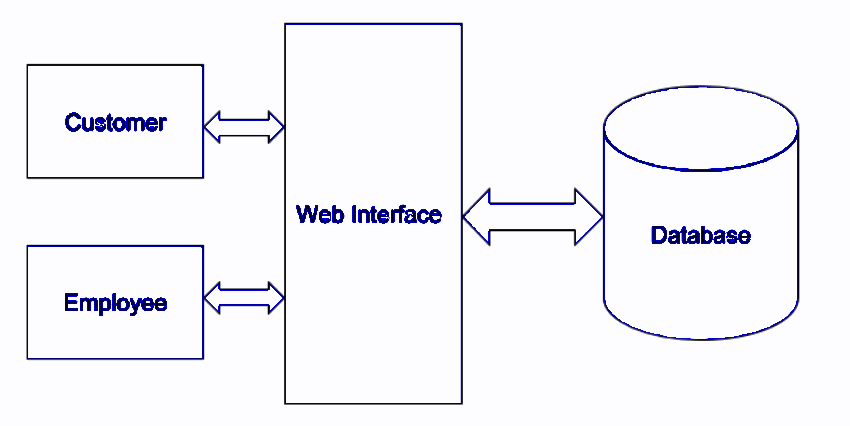
\includegraphics[scale=0.4]{arc}
\caption{System Architecture}
\label{Architecture}
\end{figure}

\begin{figure}[h!]
  \centering
  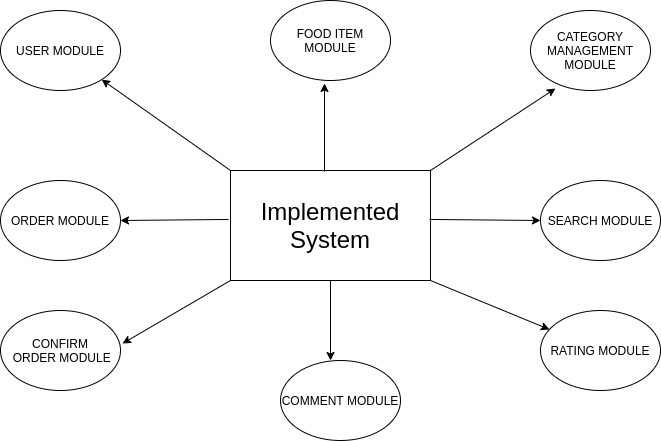
\includegraphics[scale=0.6]{mod}
  \caption{Modules Of the System}
  \label{Architecture}
  \end{figure}

\subsection{User Module}
\hspace{0.25cm}
\par
The main aim of the module is to provide all the functionalities related to the users. It tracks all the informations and details about the users. We have provided all the create, read, update and delete functionalities to this module. This is a role based module where admin can perform each and every operation on user data but users can only view his/her data. Thus access level restrictions has been implemented on the project. The admin can view the last login time of the users also.
\\
\\
\textbf{Features} :
\begin{itemize}
	\item Customer will be able to see his details.
	\item Customer will be able to update his details.
	\item All customer forms are validated on client side using Django.
	\item Only admin can edit and update the record of the customer.
	\item Admin can add new customer.
	\item Admin can see the list of customer details.
	\item Admin will be able to delete the records of the customer.
\end{itemize}

\begin{table}
  \begin{center}
    \begin{tabular}{ |c|c|c| } 
    \hline
    Field & Type  \\
    \hline
    Email\_Id & Primay Key \\
    \hline
    First\_Name & Varchar \\
    \hline
    Last\_Name & Varchar \\
    \hline
    \end{tabular}
    \caption{ User Table }
    \end{center}
  \end{table}

\subsection{Food Item Management Module}
\hspace{0.25cm}
\par
The main aim of developing this module is to manage all the deltails of the food items being served in the restaurant. So all the records of the food items can be update by the admin and the customers can view the food item lists. Also the module manages the order detail i.e the food items ordered and the details of the table no. where that food item has to be served. The customers can view the making vedio of the food item they want to order and also the daily offers are also displayed.
\\
\\
\textbf{Features :}
\begin{itemize}
	\item Admin can manage the food.
	\item Admin can edit/delete the food.
	\item Admin can see the list of all food.
	\item Customer can see food.
	\item Customers can view their placed orders.
	\item Customers can select their desired food item from the list. 
\end{itemize}

\begin{table}
  \begin{center}
    \begin{tabular}{ |c|c|c| } 
    \hline
    Field & Type  \\
    \hline
    User\_Id & Primay Key \\
    \hline
    Item & Varchar \\
    \hline
    Quantity & Integer \\
    \hline
    \end{tabular}
    \caption{ Cart Table }
    \end{center}
  \end{table}

  \begin{table}
    \begin{center}
      \begin{tabular}{ |c|c|c| } 
      \hline
      Field & Type  \\
      \hline
      User\_Id & Primay Key \\
      \hline
      Ordered\_Items & Varchar \\
      \hline
      Table\_No & Integer \\
      \hline
      \end{tabular}
      \caption{ Order Table }
      \end{center}
    \end{table}

\subsection{Category Management Module }
\hspace{0.25cm}
\par
This module manages the categories being served in the restaurant. It provides the customers an view to know the food categories available. This is categories the food items into drinks, lunch dinner, breakfast etc. This helps the customers to easily access to their favorite food item. The food items are categorised as per the admin needs. Admin can alter the category as they require. 

\textbf{Features :}
\begin{itemize}
	\item Admin can manage the item category.
	\item Admin can edit/delete the item category.
	\item Admin can see the list of all item category.
	\item Customer can see item category.
\end{itemize}

\begin{table}
  \begin{center}
    \begin{tabular}{ |c|c|c| } 
    \hline
    Field & Type  \\
    \hline
    Title\_Id & Primay Key \\
    \hline
    Primary\_Category & Boolean \\
    \hline
    \end{tabular}
    \caption{ Catrgory Table }
    \end{center}
  \end{table}

  \begin{table}
    \begin{center}
      \begin{tabular}{ |c|c|c| } 
      \hline
      Field & Type  \\
      \hline
      Object\_Id & Primay Key \\
      \hline
      Name & Varchar \\
      \hline
      Category & Integer \\
      \hline
      Detail & Varchar \\
      \hline
      Price & Varchar \\
      \hline
      \end{tabular}
      \caption{ Product Table }
      \end{center}
    \end{table}

\subsection{Confirm Order Module}
\hspace{0.25cm}
\par
The main aim of this module is provide all the functionality realted to confirm order. So all confirm order will be managed by admin and customer will be able to see confirm order. It tracks all the information and details of the confirm order.

\textbf{Features :}
\begin{itemize}
	\item Admin can add new confirm order.
	\item Admin can see the list of confirm order details.
	\item Only admin can edit and update the record of the confirm order.
	\item Admin will be able to delete the records of the confirm order.
	\item All confirm order forms are validated on client side using Django.
\end{itemize}

\begin{table}
  \begin{center}
    \begin{tabular}{ |c|c|c| } 
    \hline
    Field & Type  \\
    \hline
    User & Primay Key \\
    \hline
    Address & Varchar \\
    \hline
    ZipCode & Integer \\
    \hline
    Landmark & Varchar \\
    \hline
    \end{tabular}
    \caption{ Billing address Table }
    \end{center}
  \end{table}


\subsection{Comment Module }
\hspace{0.25cm}
\par
The main aim of developing this module is to get the feedback of the food items from customers. The number of comment of each food item is displayed to the customers. All the comments are visible to the customers.

\textbf{Features}
\begin{itemize}
	\item Costumers can comment for each food item on the list.
	\item Comment can be visible  with time and date on the Food item management module.
	\item Admin can add or delete the comments.
	\item Total number of comments is mentioned.
\end{itemize}
\par
We have developed this comments using django comments. Django includes a comments framework. This framework can be used to attach comments to any model, so you can use it for comments on blog entries, photos, book chapters, or anything else. 
\\
\\
\par
\textbf{A Roadmap of how we built this comment system}
\begin{itemize}
	\item Created a model to save the comments.
	\item Created a form to submit comments and validate the input data.
	\item Added a view that processes the form and saves the new comment to the database.
	\item Edited the post detail template to display the list of comments and the form to add a new comment.
\end{itemize}

\begin{table}
  \begin{center}
    \begin{tabular}{ |c|c|c| } 
    \hline
    Field & Type  \\
    \hline
    Object\_Id & Primay Key \\
    \hline
    Name & Varchar \\
    \hline
    Content Type & Varchar \\
    \hline
    Date-time & date \\
    \hline
    \end{tabular}
    \caption{ Comment Table }
    \end{center}
  \end{table}

\subsection{QR Code scanning }
\hspace{0.25cm}
\par
In our proposed system we provide a QR Code on every table whih will be regenerated after every 30 seconds. Scanning the QR Code the customers will be taken to our proposed website from where they can access our menu card to place their desiered order.  
\subsection{Rating Module}
\hspace{0.25cm}
\par
The main aim of this module to allow the users and admin to rate each food item.  The rating of a food item is taken as average ratings of all the customers. Admin cannot alter the ratings, the rating is dispalyed as the average rating of the all for each food item.
\newline
\par
\textbf{Features :}
\begin{itemize}
	\item Admin cannot change the rating as per their needs.
	\item We have developed an very genuine rating system.
	\item Average ratings are showcased fro each food item.
\end{itemize}

\begin{table}
\begin{center}
  \begin{tabular}{ |c|c|c| } 
  \hline
  Field & Type  \\
  \hline
  Object\_Id & Primay Key \\
  \hline
  Count & Integer \\
  \hline
  Total & Integer \\
  \hline
  Average & Integer \\
  \hline
  \end{tabular}
  \caption{ Rating Table }
  \end{center}
\end{table}

\begin{table}
  \begin{center}
    \begin{tabular}{ |c|c|c| } 
    \hline
    Field & Type  \\
    \hline
    Object\_Id & Primay Key \\
    \hline
    User & Varchar \\
    \hline
    Score & Integer \\
    \hline
    Rating & Varchar \\
    \hline
    \end{tabular}
    \caption{ User Rating Table }
    \end{center}
  \end{table}


\subsection{Payment Module }
\hspace{0.25cm}
\par
The main purpose for developing this module is to manage the customer's payment via online or cash on delivery. Admin will manage all cash on delivery record. As per the customer convenience, customer can pay their bills. Admin manages all the payment records of all the customers. 



% %chapter3-------------------------------------------------------------------------------
\chapter{IMPLEMENTATION}
\section{OVERVIEW}
\hspace{0.25cm}
\par
In this proposed system, a QR Code is regenertated for every 30 seconds. This protects the uniqueness of this project. The customers can scan the QR Code in order to access the website we have developed. The customers can pick their desired Food items from the categorised food item list. And drop into their carts. They can place the orders and pay their bills after confirming their orders. the payment can be done through the payment module or can pay on desk after the satisfactory meal. This can be done according to the customers convenience.


\section{Implemenetation of the Modules}
\hspace{0.25cm}
\par
The proposed system is majorly devepoled using the Django Framework. Django is a Python-based free and open-source web framework, which follows the model-template-view (MTV) architectural pattern. It is maintained by the Django Software Foundation (DSF), an independent organization established as a 501(c)(3) non-profit.
\\
\\
\par
Django is a Python-based free and open-source web framework, which follows the model-template-view architectural pattern. It is maintained by the Django Software Foundation, an independent organization established as a 501 non-profit. Django's primary goal is to ease the creation of complex, database-driven websites.
\\
\\
\par
Despite having its own nomenclature, such as naming the callable objects generating the HTTP responses "views",[5] the core Django framework can be seen as an MVC architecture.[6] It consists of an object-relational mapper (ORM) that mediates between data models (defined as Python classes) and a relational database ("Model"), a system for processing HTTP requests with a web templating system ("View"), and a regular-expression-based URL dispatcher ("Controller").
\\
\\
\par
Also included in the core framework are:
\begin{itemize}
	\item a lightweight and standalone web server for development and testing
	\item a form serialization and validation system that can translate between HTML forms and values suitable for storage in the database
	\item a template system that utilizes the concept of inheritance borrowed from object-oriented programming
	\item a caching framework that can use any of several cache methods
	\item an interface to Python's built-in unit test framework
	\item Django REST framework is a powerful and flexible toolkit for building Web APIs.
\end{itemize}
\par
The basic layout of the website has been developed using HTML, CSS and bootstrap. Hypertext Markup Language (HTML) is the standard markup language for documents designed to be displayed in a web browser. It can be assisted by technologies such as Cascading Style Sheets (CSS) and scripting languages such as JavaScript.

Web browsers receive HTML documents from a web server or from local storage and render the documents into multimedia web pages. HTML describes the structure of a web page semantically and originally included cues for the appearance of the document. HTML can embed programs written in a scripting language such as JavaScript, which affects the behavior and content of web pages. Inclusion of CSS defines the look and layout of content. The World Wide Web Consortium (W3C), former maintainer of the HTML and current maintainer of the CSS standards, has encouraged the use of CSS over explicit presentational HTML since 1997.

CSS is designed to enable the separation of presentation and content, including layout, colors, and fonts. This separation can improve content accessibility, provide more flexibility and control in the specification of presentation characteristics, enable multiple web pages to share formatting by specifying the relevant CSS in a separate .css file, and reduce complexity and repetition in the structural content.

\section{Implementation of Payment Module}
\hspace{0.25cm}
\par
A Payment System is a mechanism that facilitates transfer of value between a payer and a beneficiary by which the payer discharges the payment obligations to the beneficiary. Payment Systems are the medium to transfer funds from one person to another that facilitate businesses and economies.
\\
\\
\par
The main purpose for developing this module is to manage the customer's payment via online or cash on delivery. Admin will manage all cash on delivery record. As per the customer convenience, customer can pay their bills. Admin manages all the payment records of all the customers. 
\\
\\
\par
We have developed the payement module using  Stripe API. There are many payment services available in the market to integrate
payment gateway in an application. For example, PayPal, Stripe, Sage Pay, CCAvenue and
there is a long list out there. They provide API for integrating payment gateway to our
software. Here we have used Stripe Payment Gateway Integration using Django. In many
countries, Stripe is the widely used for the transactions with credit and debit cards. By using a payment gateway services / API, we can enable users to do
financial transactions with our application. When it comes to integrating a payment
gateway with our application, we need to choose a reputed provider. Because it gives trust
to the users and it is important as it involves real money.
\\
\\
\par
We can use the Stripe API in test mode, which does not affect your live data or interact with the banking networks. The API key we use to authenticate the request determines whether the request is live mode or test mode. The Stripe API differs for every account as it releases new versions and tailor functionality.
\\
\\
\par
\textbf{Errors :}
Stripe uses conventional HTTP response codes to indicate the success or failure of an API request. In general: Codes in the 2xx range indicate success. Codes in the 4xx range indicate an error that failed given the information provided (e.g., a required parameter was omitted, a charge failed, etc.). Codes in the 5xx range indicate an error with Stripe's servers (these are rare).

\begin{table}
  \begin{center}
    \caption{ HTTP STATUS CODE SUMMARY }
    \begin{tabular}{ |c|c|c| } 
    \hline
    200-OK & Everything worked as expected.  \\
    \hline
    400-Bad Request & The request was unacceptable, often due to missing a required parameter. \\
    \hline
    401-Unauthorized & No valid API key provided. \\
    \hline
    402-Request Failed & The parameters are valid but the request failed. \\
    \hline
    403-Forbidden & The API key's does not have the permission to perform the request. \\
    \hline
    404-Not Found & The requested resource dose not found. \\
    \hline
    409-Conflict & The request conflicts with another request.\\
    \hline
    429-Too Many Requests & Too many requests hit the API quickly. \\
    \hline
    500, 502, 503, 504 & Something went wrong on stripe's end. \\
    \hline
    \end{tabular}
    \end{center}
  \end{table}

\textbf{Handling Errors :}
The Client libraries available raise exceptions for many reasons, such as a failed charge, invalid parameters, authentication errors, and network unavailability. It recommends writing code that gracefully handles all possible API exceptions.

\begin{table}
  \begin{center}
    \caption{ ERROR TYPES }
    \begin{tabular}{ |c|c|c| } 
    \hline
    api\_connection\_error & Failure to connect stripe's api.  \\
    \hline
    api\_error & API errors cover any other type problem and are extremely uncommon. \\
    \hline
    authentication\_error & Failure to properly authenticate yourself in the request. \\
    \hline
    card-error & most common type of error occurs user enters a card that can be charged. \\
    \hline
    rate\_limit\_error & Too many requests hit the API quickly. \\
    \hline
    invalid\_request\_error & This error arises when the request has invalid parameters. \\
    \hline
    \end{tabular}
    \end{center}
  \end{table}

\textbf{Idempotent Requests :}The API supports idempotency for safely retrying requests without accidentally performing the same operation twice. This is useful when an API call is disrupted in transit and you do not receive a response. For example, if a request to create a charge does not respond due to a network connection error, you can retry the request with the same idempotency key to guarantee that no more than one charge is created. To perform an idempotent request, provide an additional idempotency\_key element to the request options. Stripe's idempotency works by saving the resulting status code and body of the first request made for any given idempotency key, regardless of whether it succeeded or failed. Subsequent requests with the same key return the same result, including 500 errors. 
\\
\\
\par
An idempotency key is a unique value generated by the client which the server uses to recognize subsequent retries of the same request. How you create unique keys is up to you, but we suggest using V4 UUIDs, or another random string with enough entropy to avoid collisions. Keys are eligible to be removed from the system after they're at least 24 hours old, and a new request is generated if a key is reused after the original has been pruned. The idempotency layer compares incoming parameters to those of the original request and errors unless they're the same to prevent accidental misuse. Results are only saved if an API endpoint started executing. If incoming parameters failed validation, or the request conflicted with another that was executing concurrently, no idempotent result is saved because no API endpoint began execution. It is safe to retry these requests. All POST requests accept idempotency keys. Sending idempotency keys in GET and DELETE requests has no effect and should be avoided, as these requests are idempotent by definition.



\section{Implementation of Social Authentication}
\hspace{0.25cm}
\par
Adding Social Authentication to Django. Python Social Auth is a library that provides “an easy-to-setup social authentication / registration mechanism with support for several frameworks and auth providers”.
Django comes with a user authentication system. It handles user accounts, groups, permissions and cookie-based user sessions. The Django authentication system handles both authentication and authorization. Briefly, authentication verifies a user is who they claim to be, and authorization determines what an authenticated user is allowed to do. Here the term authentication is used to refer to both tasks.
\\
\\
\par
The auth system consists of:
\begin{itemize}
  \item Users
  \item Permissions: Binary (yes/no) flags designating whether a user may perform a certain task.
  \item Groups: A generic way of applying labels and permissions to more than one user.
  \item A configurable password hashing system
  \item Forms and view tools for logging in users, or restricting content
  \item A pluggable backend system
\end{itemize}
\par
Python Social Auth aims to be an easy\-to\-setup social authentication and authorization mechanism for Python projects supporting protocols like OAuth (1 and 2), OpenID and others.
The initial codebase is derived from django-social-auth with the idea of generalizing the process to suit the different frameworks around, providing the needed tools to bring support to new frameworks.
django-social-auth itself was a product of modified code from django-twitter-oauth and django-openid-auth projects.



\section{Implementation of Django Filters}
\hspace{0.25cm}
\par
Django-filter is a generic, reusable application to alleviate writing some of the more mundane bits of view code. Specifically, it allows users to filter down a queryset based on a model's fields, displaying the form. Django-filter provides a simple way to filter down a queryset based on parameters a user provides. 



\section{Implementation of QR Code Scanning}
\hspace{0.25cm}
\par
In our proposed system, QR code Scanning is the first step to access our web page. By simply
scanning the provided Qr code. After which the customers can accesses our web page
easily. There is no need to download any application form the play store and also no need
to search for our website over the internet. To maintain the uniqueness of the code the QR Code is regenerated every 30 seconds.
\\
\\
\par
A QR Code is a machine-readable code consisting of an array of black and
white squares, typically used for storing URLs or other information for reading by the
camera on a smartphone.A QR code (short for "quick response" code) is a type of
barcode that contains a matrix of dots. It can be scanned using a QR scanner or a
smartphone with built-in camera. Basically, a QR code works in the same way as a
barcode at the supermarket. It is a machine-scannable image that can instantly be read
using a Smartphone camera. Every QR code consists of a number of black squares and
dots which represent certain pieces of information.
\\
\\\par
All QR codes have a square shape and include three square outlines in the bottom-left, top-left, and top-right corners. These square outlines define the orientation of the code. The dots within the QR code contain format and version information as well as the content itself. QR codes also include a certain level of error correction, defined as L, M, Q, or H. A low amount of error correction (L) allows the QR code to contain more content, while higher error correction (H) makes the code easier to scan.
\\
\\
\par
QR codes have two significant benefits over traditional UPCs – the barcodes commonly used in retail packaging. First, since QR codes are two-dimensional, they can contain significantly more data than a one-dimensional UPC. While a UPC may include up to 25 different characters, a 33x33 (version 4) QR code, can contain 640 bits or 114 alphanumeric characters. A 177x177 (version 40) QR code can store up to 23,648 bits or 4,296 characters.
\\
\\
\par
Another advantage of QR codes is that they can be scanned from a screen. Standard UPC scanners use a laser to scan barcodes, which means they typically cannot scan a UPC from a screen (like a smartphone). QR scanners, however, are designed to capture 2D images printed on paper or displayed on a screen. This makes it possible to use a QR code on your smartphone as a boarding pass at the airport or as a ticket for an event.
\\
\\
\par
This feautre is implemented using JavaScript and Jquery. 
The QR code of the proposed system and the add-ons are developed using JavaScript. JavaScript s a programming language that conforms to the ECMAScript specification.[7] JavaScript is high-level, often just-in-time compiled, and multi-paradigm. It has curly-bracket syntax, dynamic typing, prototype-based object-orientation, and first-class functions.Alongside HTML and CSS, JavaScript is one of the core technologies of the World Wide Web. JavaScript enables interactive web pages and is an essential part of web applications. The vast majority of websites use it for client-side page behavior, and all major web browsers have a dedicated JavaScript engine to execute it.
\\
\\
\par
As a multi-paradigm language, JavaScript supports event-driven, functional, and imperative programming styles. It has application programming interfaces (APIs) for working with text, dates, regular expressions, standard data structures, and the Document Object Model (DOM). However, the language itself does not include any input/output (I/O), such as networking, storage, or graphics facilities, as the host environment (usually a web browser) provides those APIs.
\\
\\
\par
JavaScript (JS) is a lightweight, interpreted, or just-in-time compiled programming language with first-class functions. While it is most well-known as the scripting language for Web pages, many non-browser environments also use it, such as Node.js, Apache CouchDB and Adobe Acrobat. JavaScript is a prototype-based, multi-paradigm, single-threaded, dynamic language, supporting object-oriented, imperative, and declarative (e.g. functional programming) styles. Read more about JavaScript.
\\
\\
\par
jQuery is a JavaScript library designed to simplify HTML DOM tree traversal and manipulation. jQuery's syntax is designed to make it easier to navigate a document, select DOM elements, create animations, handle events, and develop Ajax applications. jQuery also provides capabilities for developers to create plug-ins on top of the JavaScript library. This enables developers to create abstractions for low-level interaction and animation, advanced effects and high-level, themeable widgets. The modular approach to the jQuery library allows the creation of powerful dynamic web pages and Web applications.
\\
\\\par
jQuery also provides a paradigm for event handling that goes beyond basic DOM element selection and manipulation. The event assignment and the event callback function definition are done in a single step in a single location in the code. jQuery also aims to incorporate other highly used JavaScript functionality (e.g. fade ins and fade outs when hiding elements, animations by manipulating CSS properties). The jQuery library is typically distributed as a single JavaScript file that defines all its interfaces, including DOM, Events, and Ajax functions. It can be included within a Web page by linking to a local copy, or by linking to one of the many copies available from public servers. jQuery has a content delivery network (CDN) hosted by MaxCDN.

\section{Creating Databases}
\hspace{0.25cm}
\par
In the proposed system the databases has been created using ProstgreSQL. PostgreSQL is a free and open-source relational database management system (RDBMS) emphasizing extensibility and SQL compliance. PostgreSQL features transactions with Atomicity, Consistency, Isolation, Durability (ACID) properties, automatically updatable views, materialized views, triggers, foreign keys, and stored procedures. t is designed to handle a range of workloads, from single machines to data warehouses or Web services with many concurrent users. It is the default database for macOS Server.
\\
\\
\par
PostgreSQL manages concurrency through multiversion concurrency control (MVCC), which gives each transaction a "snapshot" of the database, allowing changes to be made without affecting other transactions. This largely eliminates the need for read locks, and ensures the database maintains ACID principles. PostgreSQL offers three levels of transaction isolation: Read Committed, Repeatable Read and Serializable. Because PostgreSQL is immune to dirty reads, requesting a Read Uncommitted transaction isolation level provides read committed instead. PostgreSQL supports full serializability via the serializable snapshot isolation (SSI) method.
\\
\\
\par
In PostgreSQL, a schema holds all objects, except for roles and tablespaces. Schemas effectively act like namespaces, allowing objects of the same name to co-exist in the same database. By default, newly created databases have a schema called public, but any further schemas can be added, and the public schema isn't mandatory. A search\_path setting determines the order in which PostgreSQL checks schemas for unqualified objects (those without a prefixed schema). By default, it is set to \$user, public (\$user refers to the currently connected database user). This default can be set on a database or role level, but as it is a session parameter, it can be freely changed (even multiple times) during a client session, affecting that session only.

\section{Deploying the Proposed System}
\hspace{0.25cm}
\par
The proposed system is depoyed on heroku. Heroku is a cloud platform as a service (PaaS) supporting several programming languages. One of the first cloud platforms, Heroku has been in development since June 2007, when it supported only the Ruby programming language, but now supports Java, Node.js, Scala, Clojure, Python, PHP, and Go. For this reason, Heroku is said to be a polyglot platform as it has features for a developer to build, run and scale applications in a similar manner across most languages.
\\
\\
\par
Developers use Heroku to deploy, manage, and scale modern apps. The platform is elegant, flexible, and easy to use, offering developers the simplest path to getting their apps to market. Heroku is fully managed, giving developers the freedom to focus on their core product without the distraction of maintaining servers, hardware, or infrastructure. The Heroku experience provides services, tools, workflows, and polyglot support—all designed to enhance developer productivity.
\\
\\
\par
Heroku's free cloud services begins with the apps - apps which can be deployed to dynos - the lightweight Linux containers that are at the heart of the Heroku platform. When the user sign up with Heroku, you automatically get a pool of free dyno hours to use for the apps
lications. When the application runs, it consumes dyno hours.
\\
\\
\par
Heroku gives a set of powerful capabilities that deliver higher-order value. The Heroku platform is fully-managed, meaning that it takes care of servers, hardware, and infrastructure, so that it can stay focused on the application. The platform’s flexibility allows to build apps using the preferred language or framework, and using popular architectural patterns, such as microservices.
Deploying apps on Heroku is fast and streamlined, with built-in workflows that support continuous integration and continuous delivery practices. The platform’s operational experience offers built-in tools for easily scaling and maintaining application health. Many Heroku developers use a range of free services to experiment, learn, and test out new ideas with their users before they are ready to scale.
\\
\\
\par
The required storage space while deploying the enitre project was acquired by using the Amazon Web Services (AWS). Amazon Web Services (AWS) is a subsidiary of Amazon that provides on-demand cloud computing platforms and APIs to individuals, companies, and governments, on a metered pay-as-you-go basis. In aggregate, these cloud computing web services provide a set of primitive abstract technical infrastructure and distributed computing building blocks and tools. One of these services is Amazon Elastic Compute Cloud, which allows users to have at their disposal a virtual cluster of computers, available all the time, through the Internet. AWS's version of virtual computers emulate most of the attributes of a real computer, including hardware central processing units (CPUs) and graphics processing units (GPUs) for processing; local/RAM memory; hard-disk/SSD storage; a choice of operating systems; networking; and pre-loaded application software such as web servers, databases, and customer relationship management (CRM).
\\
\\
\par
Amazon Simple Storage Service (S3) is a “highly durable and available store” that is ideal for storing application content such as media files, static assets, and user uploads. S3 allows you to offload the storage of static files from your app. This is crucial on Heroku, because your app’s dynos have an ephemeral filesystem. This means that all files that aren’t part of your application’s slug are lost whenever a dyno restarts or is replaced (this happens at least once daily).
\\
\\
\par
All files in S3 are stored in buckets. Buckets act as a top-level container, much like a directory. All files sent to S3 belong to a bucket, and a bucket’s name must be unique across all of S3. Access to the S3 API is governed by an Access Key ID and a Secret Access Key. The access key identifies your S3 user account, and the secret key is a password-like credential that should be stored securely.
\\
\\

% \subsection{Creating Database}

\chapter{RESULTS}
\hspace{0.25cm}
\par
The advancement in data and communication technology has greatly influenced the
business transactions. In earlier days, food industry has lagged behind alternative industries in
adopting new technology. But speedy advances in technology and heightened expectations of
customers and have forced the food industry to bring new innovative methods. Nowadays, the
adoption of wireless technology and emergence of mobile devices has a big role within the food
industry. The business and services in restaurants are often improved with the mixture of wireless
and mobile technologies. The competition in restaurants with regard to business has redoubled
with the advancements in food ordering techniques. In this paper, a digital menu card for
restaurants and ordering system using QR code scanning is proposed which is able to streamline
the operations to meet customer’s expectations. A flexible restaurant manage system which helps
you to be more systematic and quick in your services to customers. The implementation of
proposed application uses HTML/CSS and Java as the front end and at the backend
Python, Django Framework along with MySQL database is used.



\chapter{FUTURE SCOPE}
\hspace{0.25cm}
\par
In current formal dining environments, some form of physical
static menu is utilized to convey the available food and beverage
choices to customers. Said menus are generally paper based and
hence impose restrictions on the textual real estate available and
the ability a restaurateur has to update them. This document
specifies the requirements for a restaurant paper menu and
ordering replacement strategy to alleviate the problems
associated with the current archaic method.
\\
\\
\par
The existing system is paper based. The traditional menu cards
in the restaurants are paper based. Waiters use paper to write the
order of customers. The records are stored on paper. As with
anything paper based, it is so easy for things to get damaged by
Coffee stains etc, or paper being lost due to fire or accidents or
just generally lost. There is wastage of time, money, and paper.
As traditional menu cards are paper based, any changes that need
to be made in the menu card will lead to wastage. As it will
require reprinting of all the menu cards. Also, for small changes
it is not possible to print all the menu cards again and again.
There is no power to dynamically make any changes in the menu
card. To access a particular record from the stack of papers is not
efficient. From the customer’s point of view, this system is time
consuming. As, one has to wait until the waiter comes to take the
order, one has to call waiter number of times till he notices it,
there can be misinterpretation while the waiter is writing your
order on paper, and it might be possible that you are served with
a wrong dish.
\\
\\
\par
There has been improvements in the management of restaurants. Each waiter is assigned a group of tables, after
taking orders for a table the waiters enter the orders (a list of
dishes and drinks ordered by the diner or group of diners) into
the system at the PC. The waiter usually knows of any dishes that
are unavailable before taking an order. The system must confirm
the availability of dishes. Should an item not be available the
system must allow the waiter to change or even delete a
customer’s order. Dishes to be prepared are sent to the kitchen,
drinks orders to the bar. Starters and main course orders are
usually taken together. Drinks and desert orders may be taken
separately. Kitchen staff sees the dish orders on their screen,
prepare them in an appropriate sequence and confirm preparation
to the system when complete, similarly with the bar. When a
waiter sees the completion indications on his terminal he collects
the items and takes them to the table. The waiter can also check
on the status of dish and drink orders. At the end of the meal the
waiter will have the system print a bill, and he will enter the
details of payment for it. The management can give discounts.
The system keeps track of the numbers of customers served by
each waiter and the amount of money taken by each waiter.
\\
\\
\par
There are still many areas which are not closely
looked at. Like, making dynamic changes in the menu card, to
get rid away from the heap of paper based records, to assure the
customer that he’ll be served with what he has ordered, to get the
customer feedback on record.




\chapter{CONCLUSION}
\hspace{0.25cm}
\par
In this proposed system we have a QR Code in the menu card in each table of the
restaurant. For more details about the food stuff one can just scan the QR Code for the details.
After the QR Code scanning the customer gets into our website page displaying the menu items
and their respective price. In this page one can see athe entier detail about the food stuff selected.
The existing system of Hotel Management is manual. All the daily routines is carried out
manually and the records are maintained in the record books or the registers. The introduction of
our project will eliminate a good amount of mannual work. In this proposed restaurant menu card
system, displays the food stuffs available there and their respective prices. Along with the
displaying of food prices, the customer can also view the making of the foodstuffs. Not only the
prices are displayed, but also the making of each food stuff is made available to the customers. In
addition to these features we have an ordering system. Using this ordering system the customer
can order their preferences without waiting for the waiters. This concept is satisfactory for both
the hotel administration and the customers.
\\
\\
\par
This paper has succeeded in designing a cost effective and less manual effort needed ordering system. The proposed system helps you to Streamline your
operations to meet customer’s expectations. A flexible restaurant manage system which helps you to be more systematic and
quick in your services to customers. Its fast and time management system for customers. The paper also verified the designed system by constructing and testing a prototype of the system using the components outlined in this paper. 


%-----------------REFERENCES------------------------------------------------------------------------------


\begin{thebibliography}{99}
\renewcommand{\bibname}{References}
\addcontentsline{toc}{chapter}{\MakeUppercase{References}}

\bibitem{}  Ward, Paul T. "The transformation schema: An
extension of the data flow diagram to represent
control and timing." Software Engineering, IEEE
Transactions on 2 (1986): 198-210.
 
\bibitem{}Fowler, Remy J., and Will E. Leland. "Local area
network characteristics, with implications for
broadband network congestion management."
Selected Areas in Communications, IEEE Journal on
9.7 (1991): 1139-1149.
\bibitem{} Wang, Zhikui, and Fernando Paganini. "Global
stability with time-delay in network congestion
control." Decision and ControL 2002, Proceedings of
the 41stIEEE Conference on. Vol. 4. IEEE, 2002.
[8] Berman, Keith, et al. "Automated networked serv
\bibitem{} Awojide, Simon, I. M. Omogbhemhe, O. S. Awe, and T. S.
Babatope, “Towards the digitalization of Restaurant Business
Process for Food Ordering in Nigeria Private University: The
Design Perspective. A Study of Samuel Adegboyega
University Edo State Nigeria,” Int. J. Sci. Res. Publ., vol. 8,
no. 5, pp. 46–54, 2018.

\bibitem{}  Varsha Chavan, Priya Jadhav, Snehal Korade, Priyanka Teli,
”Implementing Customizable Online Food Ordering System
Using Web Based Application”, International Journal of
Innovative Science, Engineering Technology(IJISET) 2015.

\bibitem{} Tennenhouse, David L., and David 1. Wetherall.
"Towards an active network architecture." DARPA
Active Networks Conference and Exposition, 2002.
\bibitem{}Schneider, Eric. "Method, product, and apparatus for
processing a data request." U. S. Patent No.6,760,746.
6 Jul. 2004.
\end{thebibliography}

\begin{appendices}
	\chapter{Source Code}
	\begin{lstlisting}[language=HTML]






<div class="container my-5">

    
<div class="card">
    <div class="row">
        <aside class="col-sm-5 border-right">
<article class="gallery-wrap"> 
<div class="img-big-wrap">
  <div> <a href="#"><img src="/media/{{ object.mainimage }}" style="width: 450px"></a></div>
</div> <!-- slider-product.// -->
</article> <!-- gallery-wrap .end// -->
        </aside>
        <aside class="col-sm-7">
<article class="card-body p-6">
    <h3 class="title mb-3">{{ object.name }}</h3>
<p class="price-detail-wrap"> 
    <span class="price h3 text-warning"> 
        <span class="currency">₹</span><span class="num">{{ object.price }}</span>
    </span>     
</p> <!-- price-detail-wrap .// -->
<dl class="item-property">
  <dt>Description</dt>
  <dd><p>{{ object.preview_text }}</p></dd>

</dl>

<a href="" class="btn btn-lg btn-outline-primary text-uppercase"> <i class="fas fa-shopping-cart"></i> Add to cart </a>
</article> <!-- card-body.// -->
<br><br>
<h3 class="title mb-3">Making Video of {{ object.name }}</h3>

        <video width='400' controls>
        <source src='{{ MEDIA_URL }}{{ object.videofile }}' type='video/mp4'>
        Your browser does not support the video tag.
        </video>
        <br><br>
         <!-- col.// -->
    </div> <!-- row.// -->
</aside>
    
    <br><br>    

</div> <!-- card.// -->


</div>
<!--container.//-->



 
 
 
<div class="container mt-5">
  <h2 class="mb-3">Le cafe ' > <span class="text-muted">Checkout</span></h2>
  
  <div class="col-md-3">
    <div class="card" style="height: auto">
      <div class="card-body">
        <ul class="list-group list-group-flush">
          
          <li class="list-group-item">
            {{ item.item.name }} x {{ item.quantity }}
          </li>
          
        </ul>
      </div>

      <div class="card-footer">
        <span class="float-left"><b>Order Total</b></span>
        <span class="float-right"
          ><b>₹ {{ order_total | floatformat:2 }}</b></span
        >
      </div>
    </div>
    <div class="card mb-5" style="height: auto">
      <div class="card-body">
        <a href="  " class="btn btn-primary float-right">Proceed to Checkout </a>
     </div>
    </div>
  </div>
</div>






<div class="container mt-5">
<h2 class="text-center"><strong>Your Ordes</strong></h2>
<div class="row">
    <div class="col-md-12">
        <div class="card mt-5" style="height: auto">
            <div class="table-responsive">
            <table class="table">
              <thead>
                <tr>
                  <th scope="col">#</th>
                  <th scope="col">Table_no</th>
                  <th scope="col">Products</th>
                  <th scope="col">Status</th>
                </tr>
              </thead>
              <tbody>
                
                
                
                <tr>
                  <th scope="row">{{ forloop.counter }}</th>
                  <td><a href="#">Table {{ order.table_no }}</a></td>
                  <td>
                    
                        {{ item }}
                        <br>
                    
                  </td>
                  <td><span class="badge badge-primary">Processing Your Order</span></td>
                </tr>
                  
                
              </tbody>
            </table>
            </div>
        </div>
    </div>
    <div class="col-md-12 my-5 text-center">
        <a href="/" class="btn btn-success">Back to Home</a>
    </div>
</div>
</div>



payment.html

  


<div class="container">
  <div class="jumbotron">
    <h1>Choose your payment option</h1>
  </div>
</div>
<br />
<h1 class="text-center">Grand Total: ₹ {{ tot }}</h1>
<h5 class="text-center">
  including all service charges. (no delivery charges applied)
</h5>
<br />
<div class="container mt-5 text-center">
  <h1 class="text-center">
    <a href=""
    ><button class="btn btn-warning">
      <span class="glyphicon glyphicon-circle-arrow-left"></span> Go back to
      cart
    </button></a
  >
  <form action="" method="post">
    
    
  <a 
  ><button
    type="submit"
    name="success"
    value="success"
    class="btn btn-success"
  >
    <span class="glyphicon glyphicon-"></span> Cash On Delivery
  </button></a
>

</form>
</h1>

  <form action="" method="POST">
    
   <script
      src="https://checkout.stripe.com/checkout.js"
      class=" stripe-button"
      data-key="{{ key }}"
      data-description="Complete your order"
      data-amount="{{ total }}"
      data-locale="auto"
    ></script>
  </form>
</div>
 


table.html

 
 

<div class="container mt-5">
    <div class="col-md-3">
      <div class="card" style="height: auto">
    <div class="card-body">
      <form method="POST" action="" >
        
        <label>
    
          <span class="float-left"><b>Enter Your Table No :</b></span>
          <input
            type="number"
            id="table"
            name="table"
            min="1"
            max="20"
          />
        </label>
       
        <br />
        <button type="submit" class="btn btn-success">
          submit table_number
        </button>
      </form>
    </div>
    
    </div>
    <div class="card-body">
      <a href="  " class="btn btn-primary float-right">Proceed to Checkout </a>
   </div>
    </div>
    
    </div>



home.html






<div class="container">
    <!--Slideshow starts here -->
    
    <h5 class="my-4">{{product.0.category}} - Recommended Items</h5>
    <div class="row">
        <div id="demo{{forloop.counter}}" class="col carousel slide my-3" data-ride="carousel">
            <ul class="carousel-indicators">
                <li data-target="#demo{{forloop.counter}}" data-slide-to="0" class="active"></li>
                
                <li data-target="#demo{{forloop.parentloop.counter}}" data-slide-to="{{i}}"></li>
                
            </ul>
            <div class="container carousel-inner no-padding">
                <div class="carousel-item active">
                    
                    <div class="col-xs-3 col-sm-3 col-md-3">
                        <div class="card-deck">
                            <div class="card align-items-center" style="width: 18rem;">
                                <img src='/media/{{i.mainimage}}' class="card-img-top" alt="...">
                                <div class="card-body">
                                    <h5 class="card-title" id="namepr{{i.id}}"><a href="{{ i.get_absolute_url }}">{{i.name}}</a></h5>
                                    <h6 class="card-title" >₹<span id="pricepr{{i.id}}">{{i.price}}</span></h6>
                                </div>
                            </div>
                        </div>
                    </div>
					
					    </div>
        <div class="carousel-item">
             
        </div>
    </div>
 </div>
     <!-- left and right controls for the slide -->
	<a class="carousel-control-prev" href="#demo{{forloop.counter}}" data-slide="prev">
    <span class="carousel-control-prev-icon"></span>
    </a>
	<a class="carousel-control-next" href="#demo{{forloop.counter}}" data-slide="next">
    <span class="carousel-control-next-icon"></span>
    </a>
</div>

</div>

 


home.html






<div class="container">
    <!--Slideshow starts here -->
    
    <h5 class="my-4">{{product.0.category}} - Recommended Items</h5>
    <div class="row">
        <div id="demo{{forloop.counter}}" class="col carousel slide my-3" data-ride="carousel">
            <ul class="carousel-indicators">
                <li data-target="#demo{{forloop.counter}}" data-slide-to="0" class="active"></li>
                
                <li data-target="#demo{{forloop.parentloop.counter}}" data-slide-to="{{i}}"></li>
                
            </ul>
            <div class="container carousel-inner no-padding">
                <div class="carousel-item active">
                    
                    <div class="col-xs-3 col-sm-3 col-md-3">
                        <div class="card-deck">
                            <div class="card align-items-center" style="width: 18rem;">
                                <img src='/media/{{i.mainimage}}' class="card-img-top" alt="...">
                                <div class="card-body">
                                    <h5 class="card-title" id="namepr{{i.id}}"><a href="{{ i.get_absolute_url }}">{{i.name}}</a></h5>
                                    <h6 class="card-title" >₹<span id="pricepr{{i.id}}">{{i.price}}</span></h6>
                                </div>
                            </div>
                        </div>
                    </div>
                    
                </div>
                <div class="carousel-item">
                     
                </div>
            </div>
        </div>
        <!-- left and right controls for the slide -->
        <a class="carousel-control-prev" href="#demo{{forloop.counter}}" data-slide="prev">
            <span class="carousel-control-prev-icon"></span>
        </a>
        <a class="carousel-control-next" href="#demo{{forloop.counter}}" data-slide="next">
            <span class="carousel-control-next-icon"></span>
        </a>
    </div>
    
</div>

 



	\end{lstlisting}
	\chapter{Screenshots}
	\begin{figure}[h!]
		\centering
		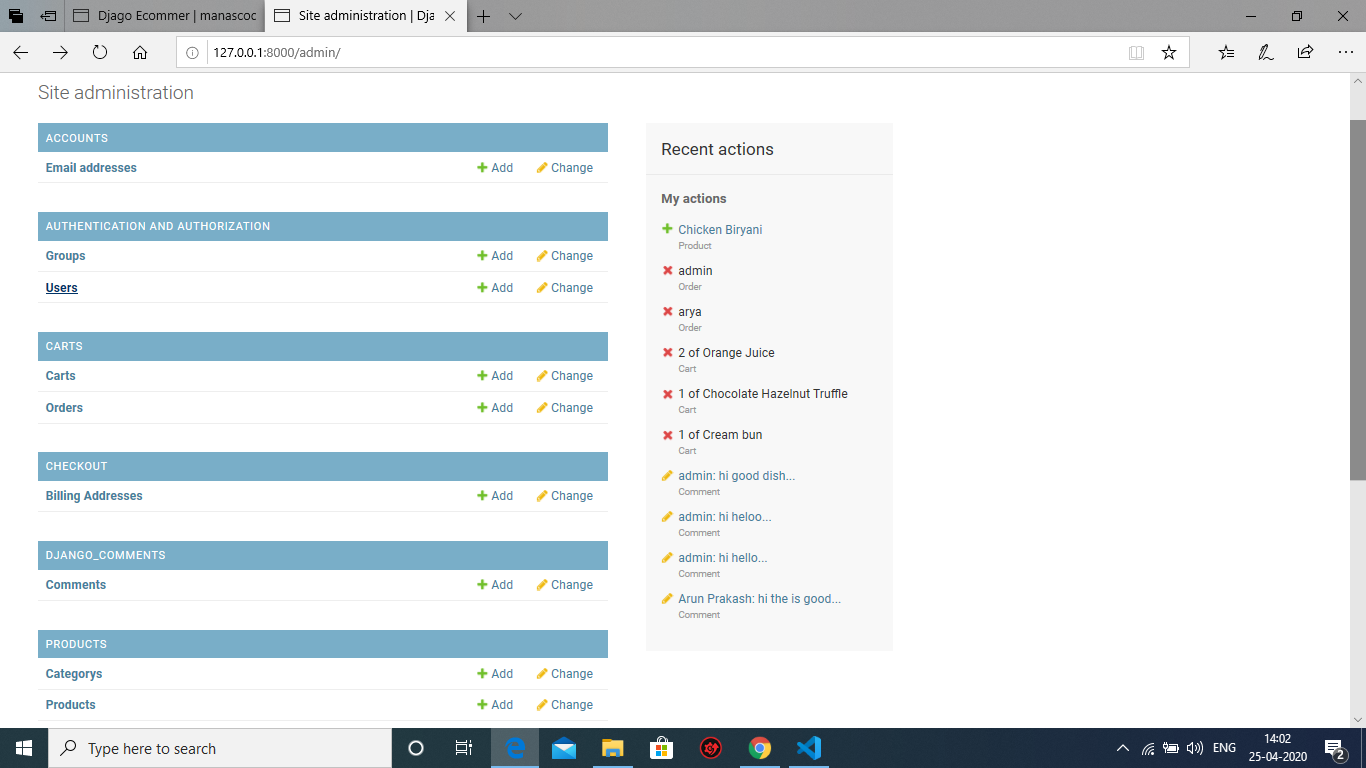
\includegraphics[scale=0.3]{12}
		\caption{System Modules}
		\label{Architecture}
		\end{figure}

\begin{figure}[h!]
	\centering
	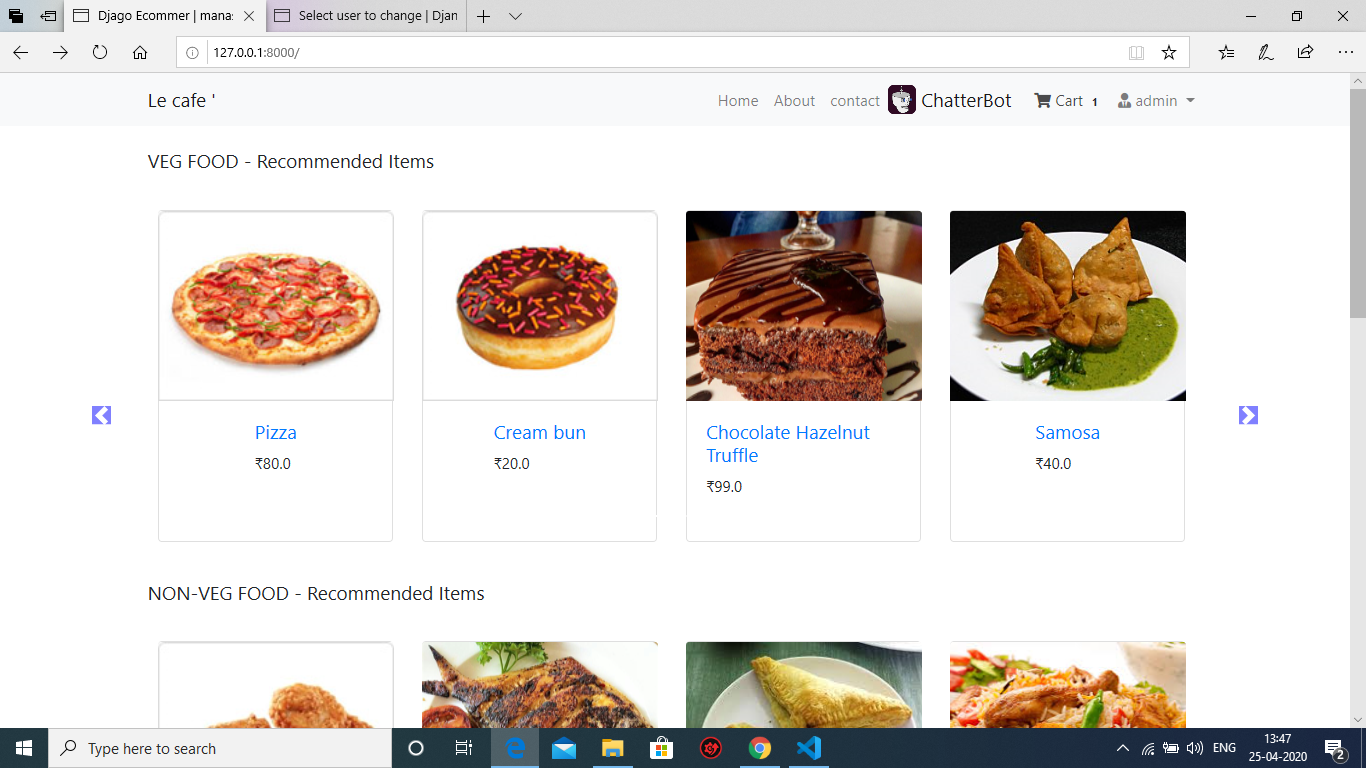
\includegraphics[scale=0.3]{1}
	\caption{Food Item Management Module}
	\label{Architecture}
\end{figure}

\begin{figure}[h!]
	\centering
	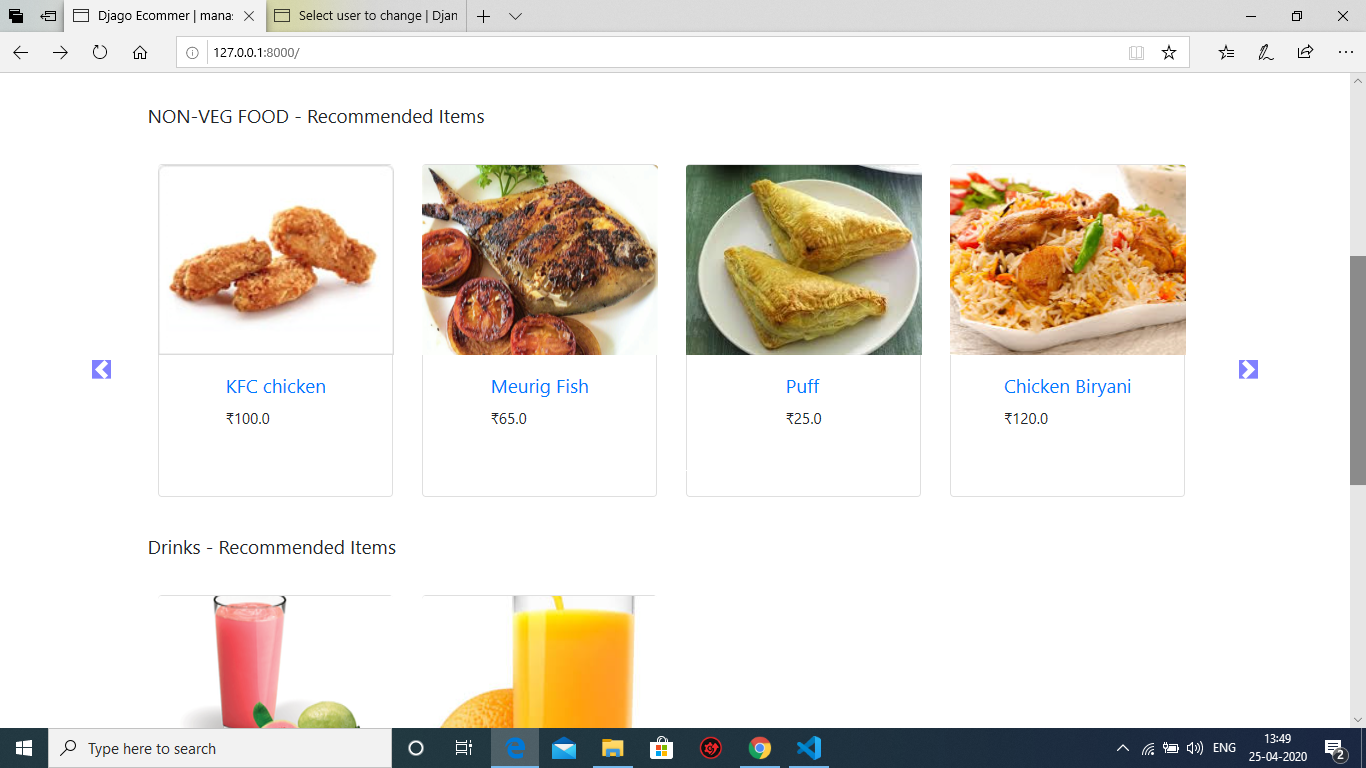
\includegraphics[scale=0.3]{2}
	\caption{Category Management Modue}
	\label{Architecture}
\end{figure}

\begin{figure}[h!]
	\centering
	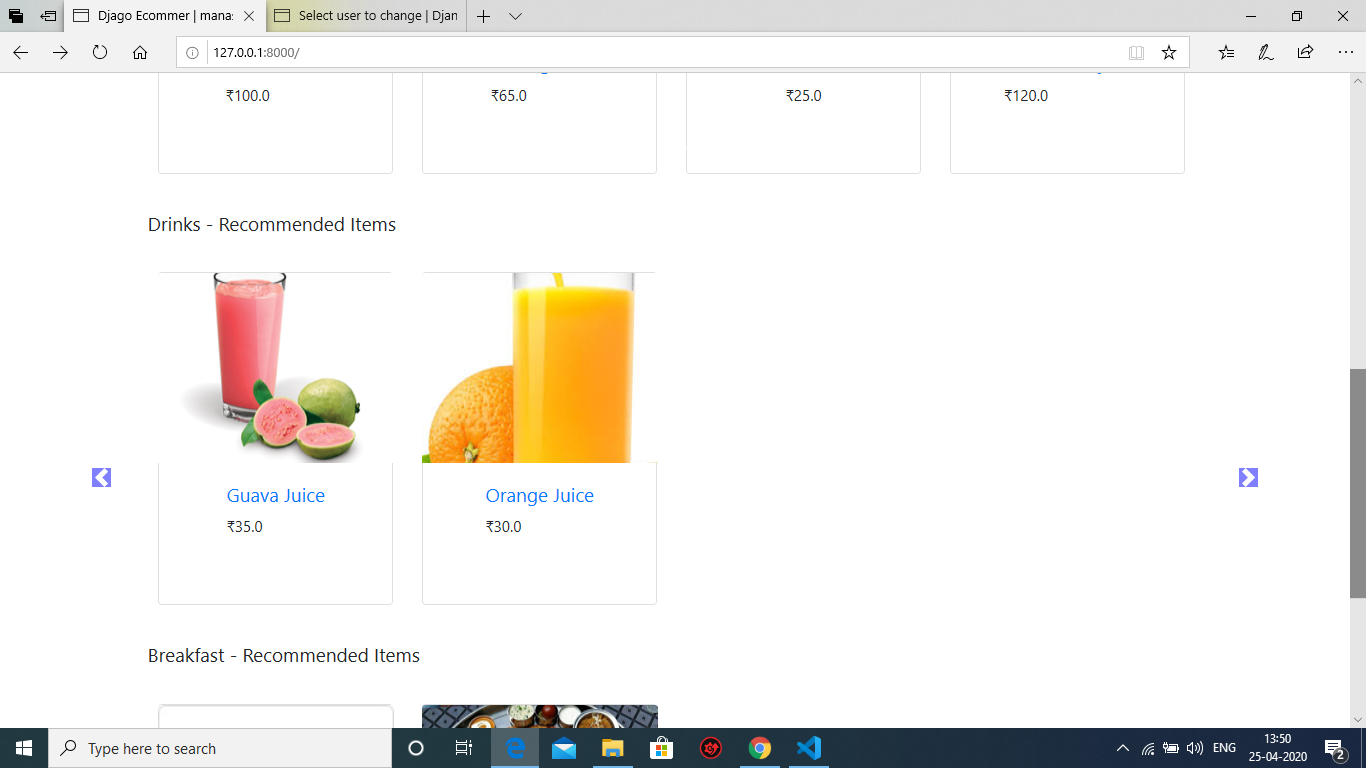
\includegraphics[scale=0.3]{3}
	\caption{Category Management Module}
	\label{Architecture}
\end{figure}

\begin{figure}[h!]
	\centering
	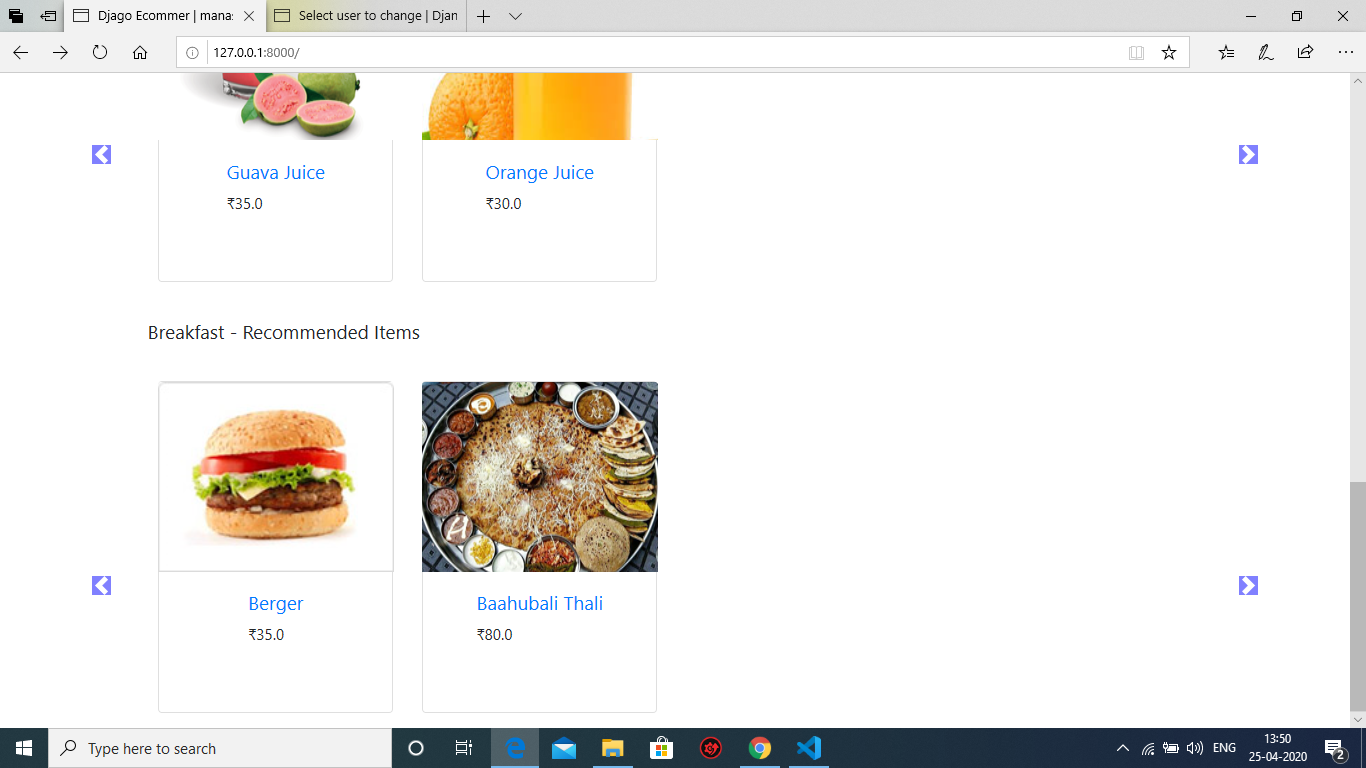
\includegraphics[scale=0.3]{4}
	\caption{Category Management Module}
	\label{Architecture}
\end{figure}

\begin{figure}[h!]
	\centering
	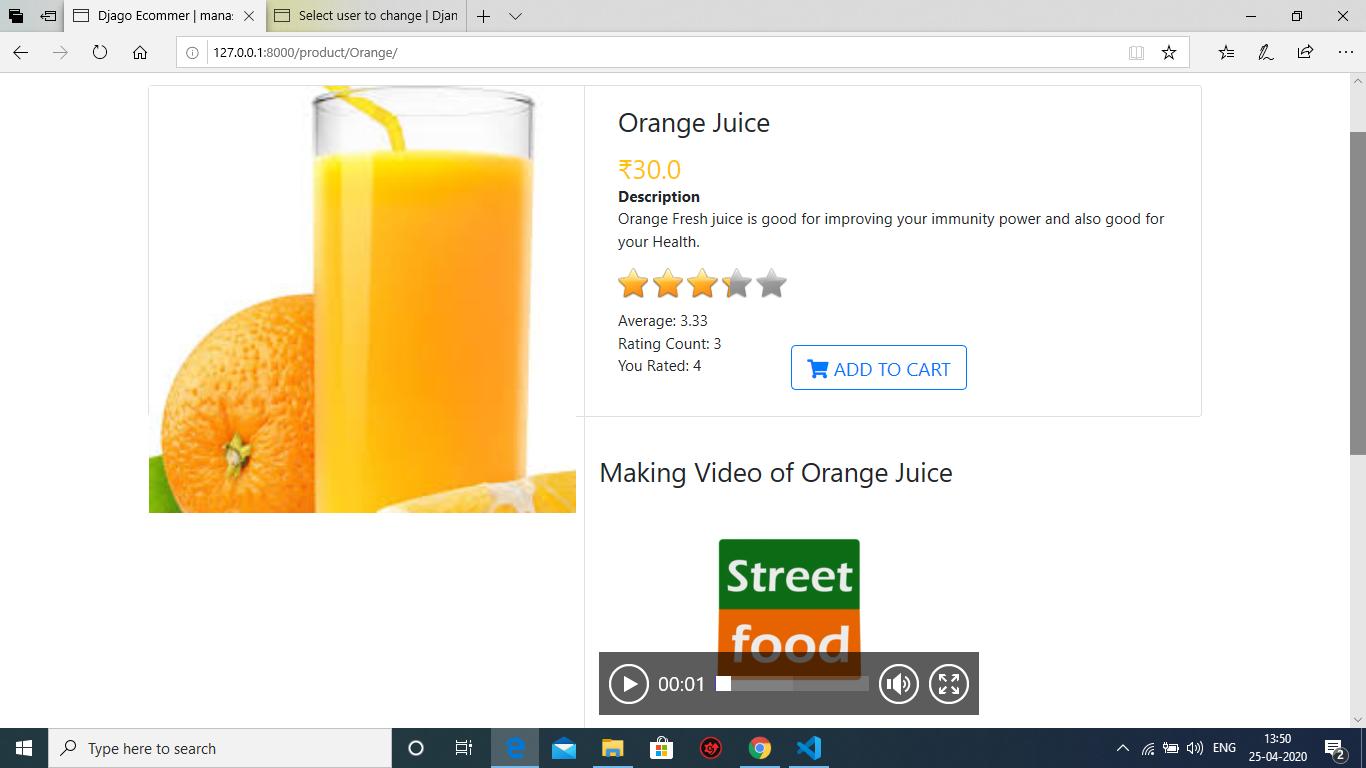
\includegraphics[scale=0.3]{5}
	\caption{Rating System}
	\label{Architecture}
\end{figure}

\begin{figure}[h!]
	\centering
	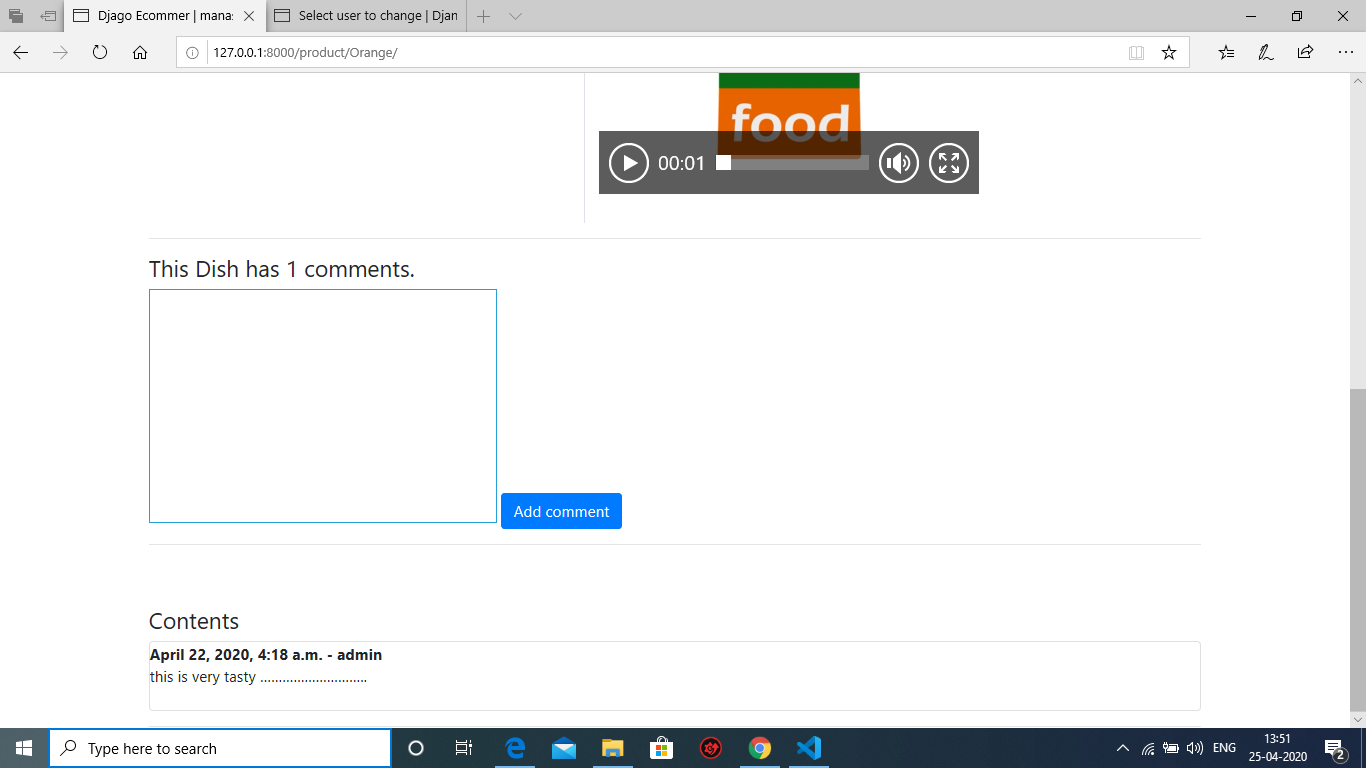
\includegraphics[scale=0.3]{6}
	\caption{Comment Area}
	\label{Architecture}
	\end{figure}

\begin{figure}[h!]
	\centering
	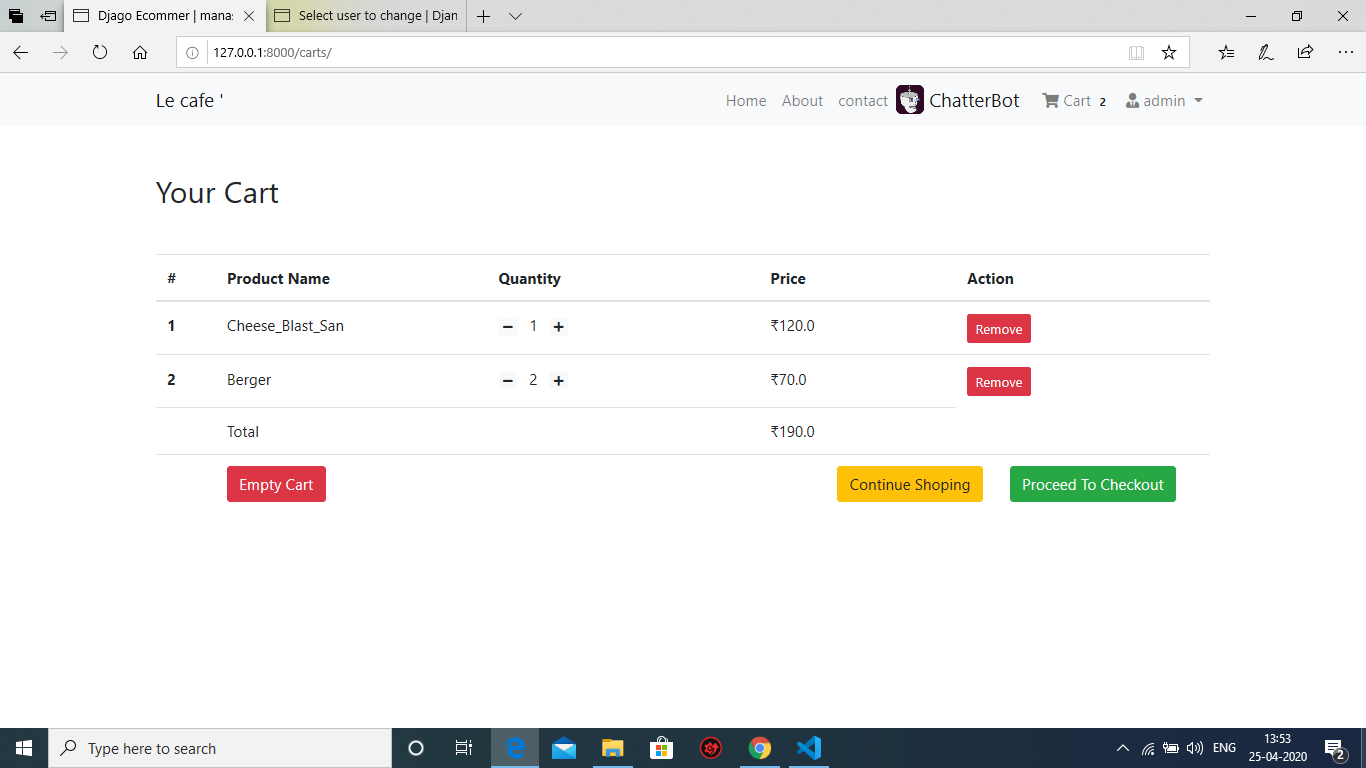
\includegraphics[scale=0.3]{7}
	\caption{Food Cart}
	\label{Architecture}
\end{figure}
		
\begin{figure}[h!]
	\centering
	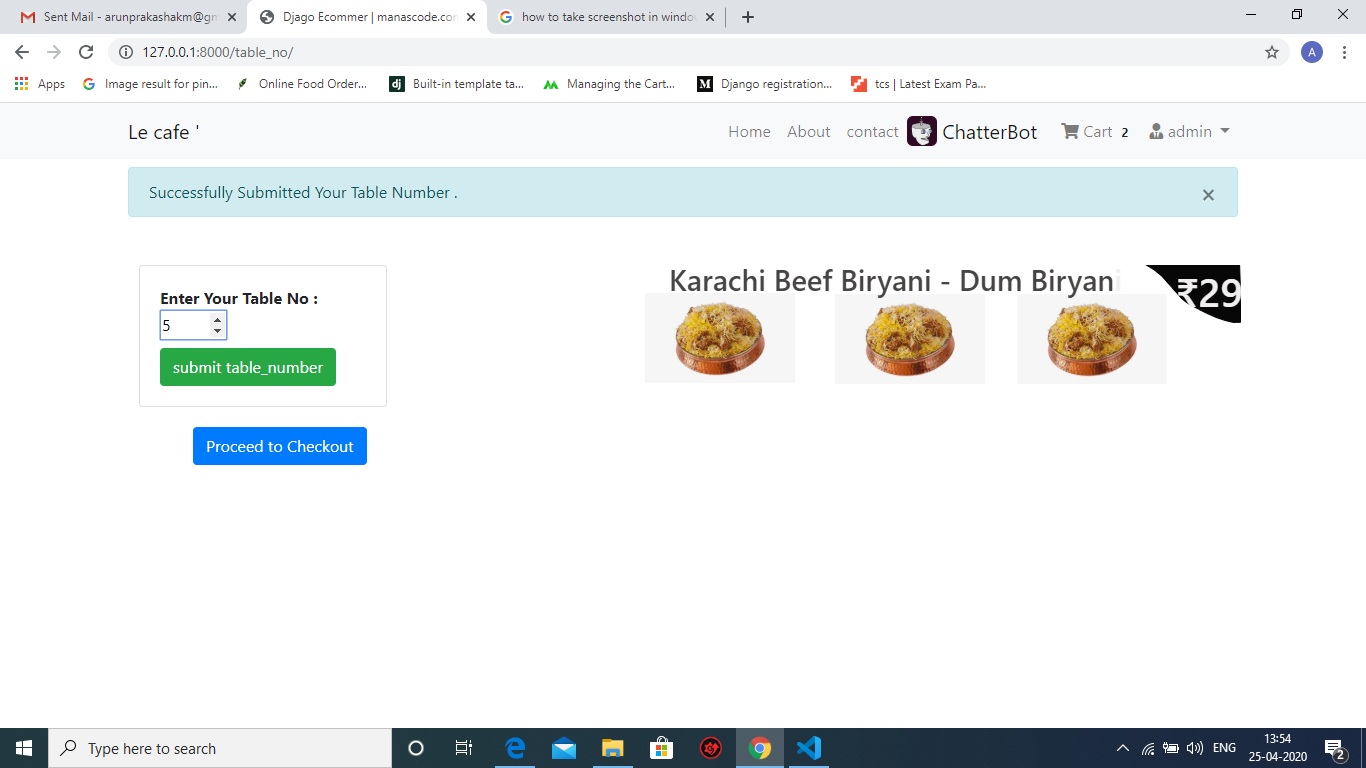
\includegraphics[scale=0.3]{8}
	\caption{Table Number Entry and Add-Ons}
	\label{Architecture}
	\end{figure}

\begin{figure}[h!]
	\centering
	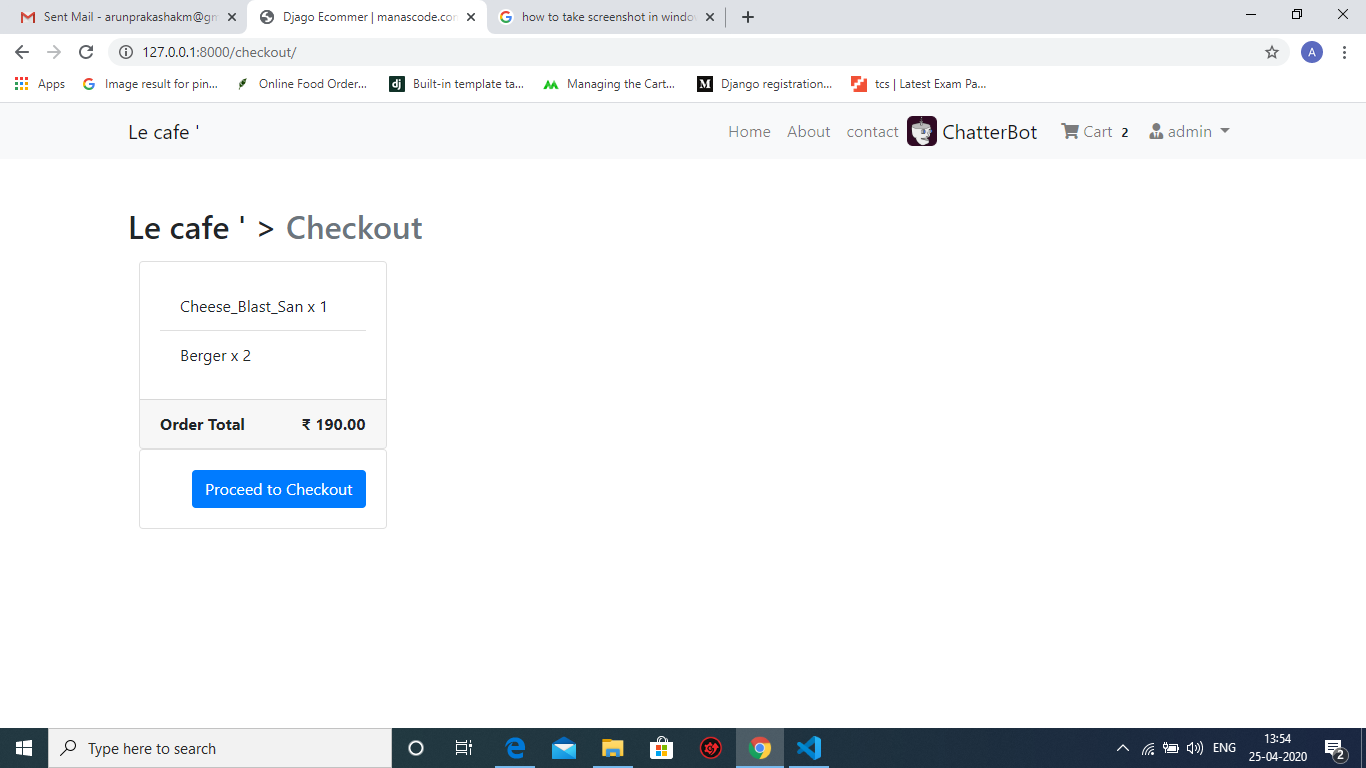
\includegraphics[scale=0.3]{9}
	\caption{Confirming Order}
	\label{Architecture}
\end{figure}	

\begin{figure}[h!]
	\centering
	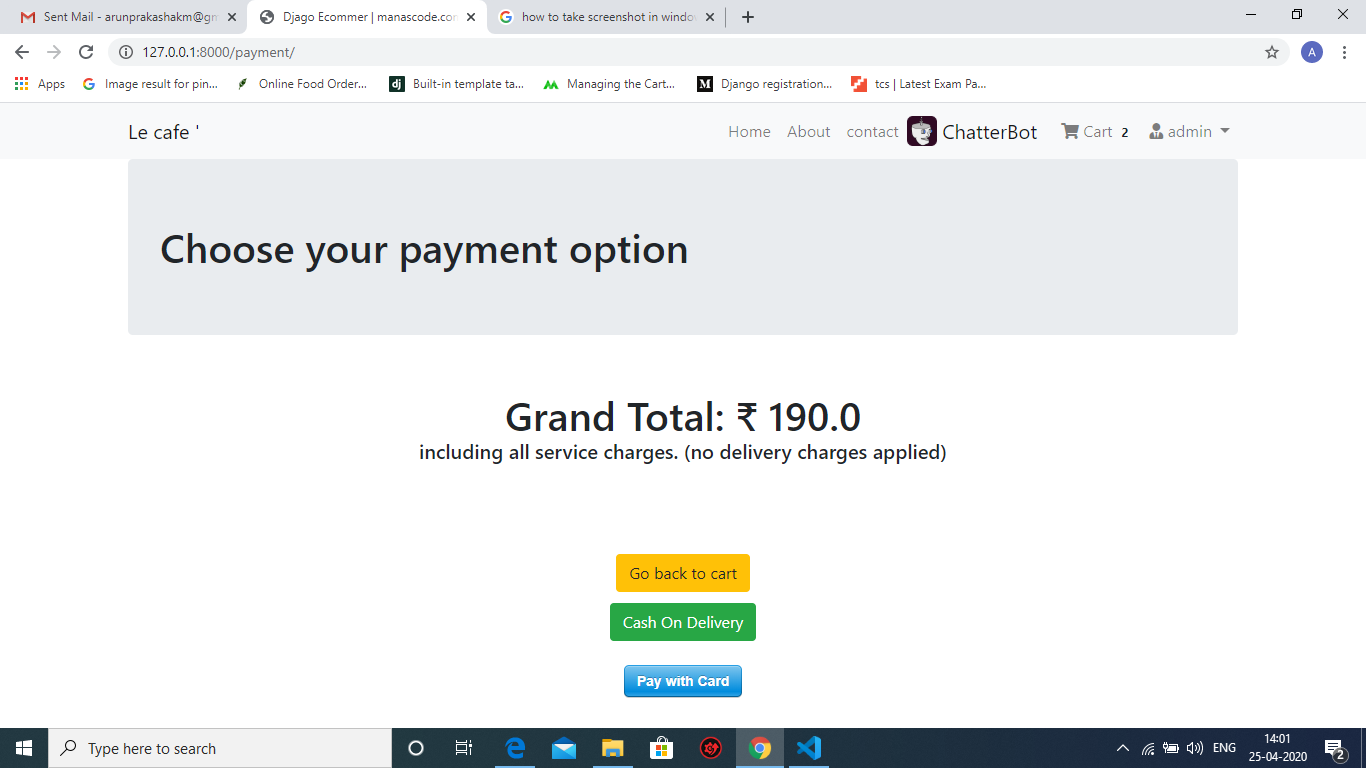
\includegraphics[scale=0.3]{10}
	\caption{Payment Module}
	\label{Architecture}
\end{figure}

\begin{figure}[h!]
	\centering
	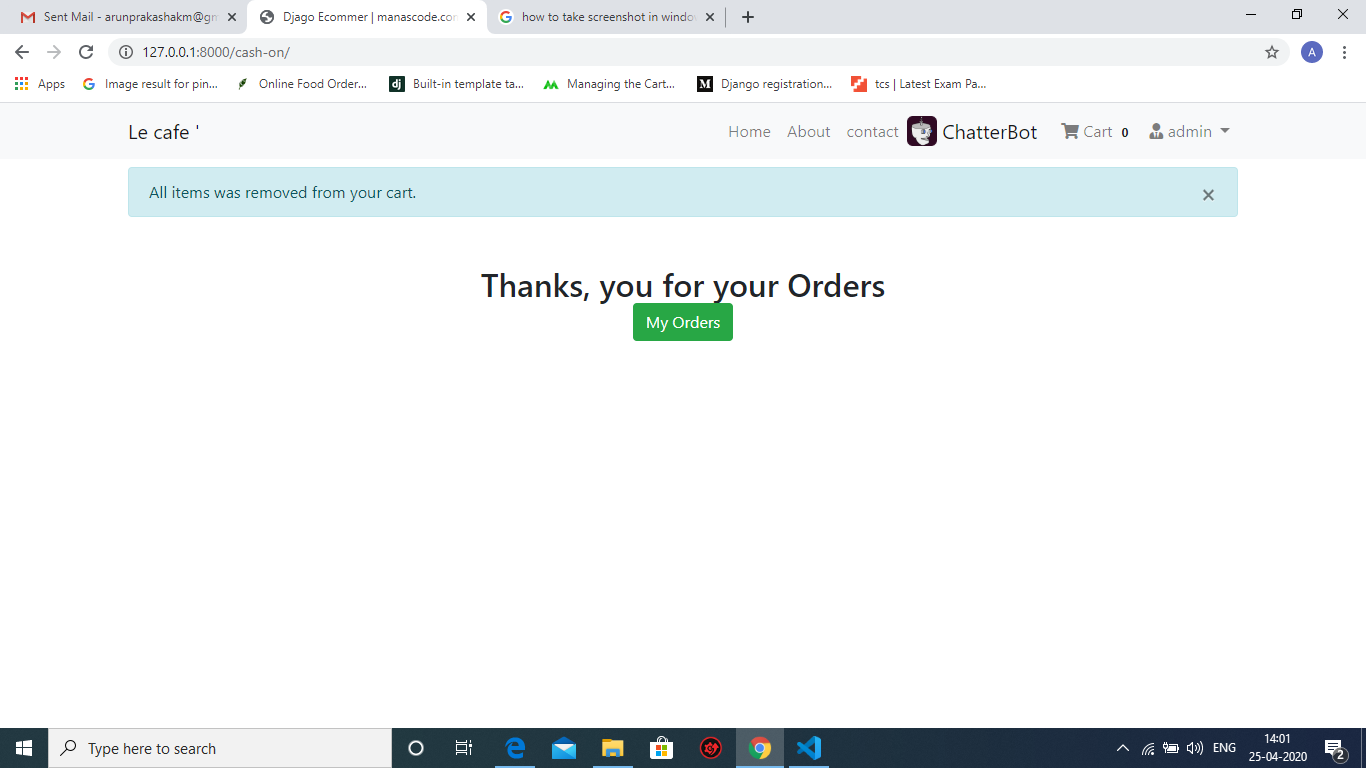
\includegraphics[scale=0.3]{11}
	\caption{Payment Module}
	\label{Confirming Order}
	\end{figure}

	\begin{figure}[h!]
		\centering
		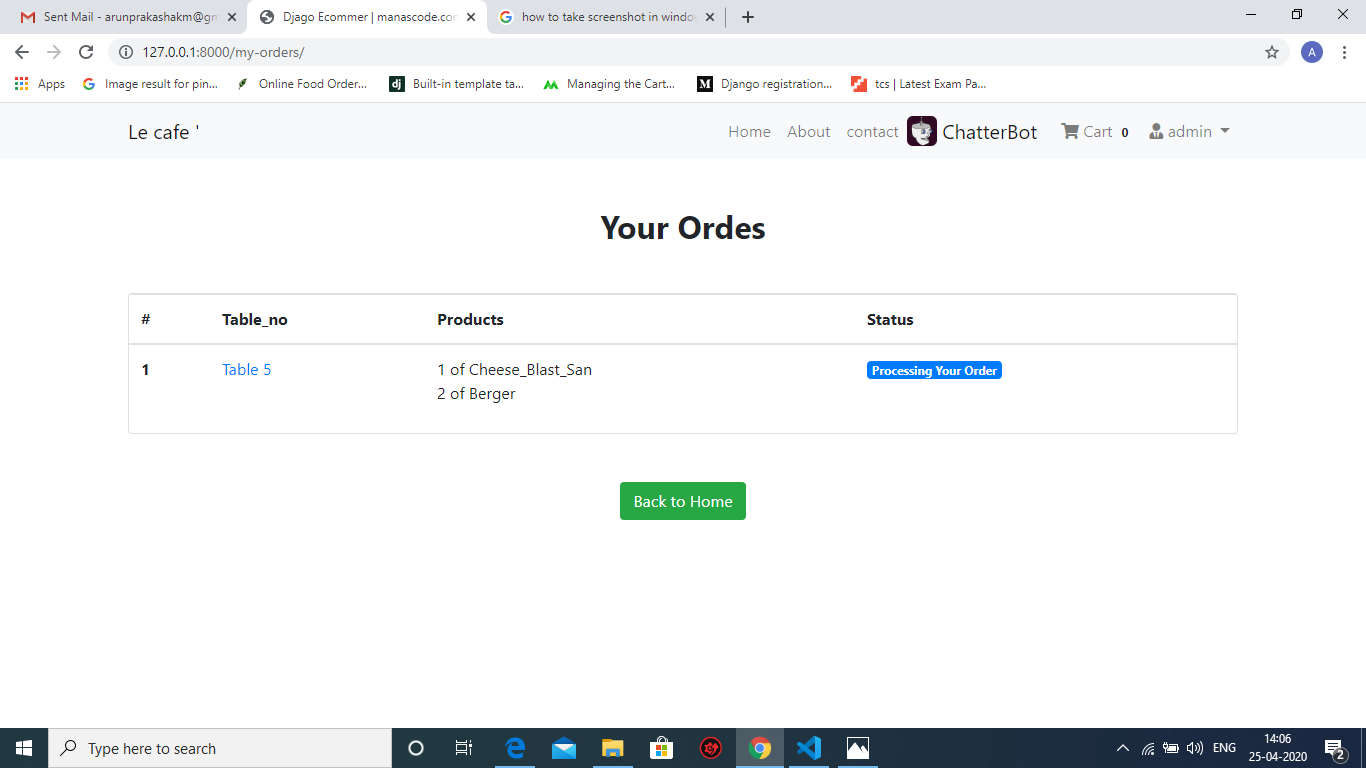
\includegraphics[scale=0.3]{13}
		\caption{Customer view of their placed Orders}
		\label{Architecture}
		\end{figure}	
	
\end{appendices}


\end{document}
